\documentclass[11pt]{article}

\usepackage[T1]{fontenc}
\usepackage[utf8]{inputenc}
\usepackage[english]{babel}
\usepackage[margin=1in]{geometry}
\usepackage{lmodern}
\usepackage{microtype}
\usepackage{mathtools}
\usepackage{amsmath,amssymb,amsthm}
\usepackage{array}
\usepackage{booktabs}
\usepackage{tabularx}
\usepackage{longtable}
\usepackage{float}
\usepackage{graphicx}
\usepackage{pdflscape}
\usepackage{caption}
\usepackage{enumitem}
\usepackage{fancyhdr}
\usepackage[numbers]{natbib}
\usepackage{doi}
\usepackage{xurl}
\usepackage{hyperref}
\usepackage{cleveref}
\usepackage{orcidlink}
\usepackage{titling}
\usepackage{xcolor}
\usepackage{tikz}
\usetikzlibrary{arrows.meta,positioning,calc,fit,backgrounds,shapes.geometric,decorations.pathreplacing}

% Shared manuscript macros for the paper.
% Keep cross-section vocabulary mechanically stable here as the draft evolves.

\newcommand{\SixBirds}{Six Birds}
\newcommand{\QMgr}{QM--GR}
\newcommand{\Deltafact}{\Delta_{\mathrm{fact}}}
\newcommand{\RecordStable}{\mathrm{RS}}
\newcommand{\PredictionOne}{Prediction~1}
\newcommand{\PredictionTwo}{Prediction~2}
\newcommand{\PredictionThree}{Prediction~3}

% Evidence-type palette used consistently by every figure (colour-blind safe).
\definecolor{evThm}{HTML}{0072B2}   % theorem (written proof)
\definecolor{evExact}{HTML}{009E73} % exact finite computation
\definecolor{evCond}{HTML}{D55E00}  % conditional construction / recognition
\definecolor{evNum}{HTML}{CC79A7}   % sampled numerics
\definecolor{evNeg}{HTML}{555555}   % negative result
\definecolor{evOpen}{HTML}{8A6D00}  % open program
\tikzset{
  ev/.style={draw, rounded corners=2pt, line width=0.7pt, align=left, inner sep=3pt,
    font=\scriptsize, text width=#1},
  ev/.default={4.55cm},
  thm/.style={ev, draw=evThm, fill=evThm!12},
  exact/.style={ev, draw=evExact, fill=evExact!12},
  cond/.style={ev, draw=evCond, fill=evCond!10},
  num/.style={ev, draw=evNum, fill=evNum!14},
  neg/.style={ev, draw=evNeg, fill=evNeg!10},
  open/.style={ev, draw=evOpen, dashed, fill=white},
  colhead/.style={font=\small\bfseries, align=center, text width=4.8cm, anchor=south},
  key/.style={draw, rounded corners=1.5pt, line width=0.7pt, minimum width=0.45cm, minimum height=0.28cm},
}


\DeclareUnicodeCharacter{00A7}{\S}
\DeclareUnicodeCharacter{039B}{\ensuremath{\Lambda}}
\DeclareUnicodeCharacter{03B4}{\ensuremath{\delta}}
\DeclareUnicodeCharacter{2013}{--}
\DeclareUnicodeCharacter{2192}{\ensuremath{\to}}
\DeclareUnicodeCharacter{2194}{\ensuremath{\leftrightarrow}}
\DeclareUnicodeCharacter{21D2}{\ensuremath{\Rightarrow}}

\newtheorem{theorem}{Theorem}[section]
\newtheorem{lemma}[theorem]{Lemma}
\newtheorem{proposition}[theorem]{Proposition}
\newtheorem{corollary}[theorem]{Corollary}
\theoremstyle{definition}
\newtheorem{definition}[theorem]{Definition}
\newtheorem{remark}[theorem]{Remark}
\providecommand{\tightlist}{%
  \setlength{\itemsep}{0pt}\setlength{\parskip}{0pt}}
\urlstyle{same}
\captionsetup{
  font=small,
  labelfont=bf,
  labelsep=period
}
\captionsetup[figure]{skip=6pt}
\crefname{theorem}{theorem}{theorems}
\Crefname{theorem}{Theorem}{Theorems}
\crefname{lemma}{lemma}{lemmas}
\Crefname{lemma}{Lemma}{Lemmas}
\crefname{proposition}{proposition}{propositions}
\Crefname{proposition}{Proposition}{Propositions}
\crefname{corollary}{corollary}{corollaries}
\Crefname{corollary}{Corollary}{Corollaries}
\crefname{definition}{definition}{definitions}
\Crefname{definition}{Definition}{Definitions}
\crefname{remark}{remark}{remarks}
\Crefname{remark}{Remark}{Remarks}
\setlist[enumerate]{leftmargin=*, itemsep=2pt, topsep=4pt}
\setlength{\droptitle}{-3.2em}
\pretitle{\begin{center}\LARGE\bfseries}
\posttitle{\par\end{center}\vspace{0.5em}}
\preauthor{\begin{center}\normalsize}
\postauthor{\par\end{center}\vspace{-0.4em}}
\predate{\begin{center}\small}
\postdate{\par\end{center}\vspace{0.6em}}
\setlength{\emergencystretch}{2em}
\clubpenalty=10000
\widowpenalty=10000
\displaywidowpenalty=10000
\interfootnotelinepenalty=10000
\allowdisplaybreaks[2]
\fancypagestyle{firstpage}{\fancyhf{}
  \fancyfoot[C]{\scriptsize Automorph Inc., Wilmington, DE, USA \quad \texttt{ioannis@automorph.io} \quad \textcopyright\ 2026 \quad CC-BY 4.0 \quad \doi{10.5281/zenodo.23120510}}
  \renewcommand{\headrulewidth}{0pt}
  \renewcommand{\footrulewidth}{0pt}
}

\title{To Kill Three Stones with Six Birds:\\ A Common Grammar for the SM, QM, and GR}
\author{Ioannis Tsiokos\,\orcidlink{0009-0009-7659-5964}}
\date{Version 1: 17 June 2026 \quad\textperiodcentered\quad Version 3: 3 October 2026}
\hypersetup{
  pdftitle={To Kill Three Stones with Six Birds: A Common Grammar for the SM, QM, and GR},
  pdfauthor={Ioannis Tsiokos},
  pdfkeywords={Six Birds Theory; emergence calculus; finite structural constructions; Standard Model gauge selection; quantum gravity; holographic entanglement},
  hidelinks
}

\begin{document}

\maketitle
\thispagestyle{firstpage}

\begin{abstract}
Can one small mathematical vocabulary organize two very different open problems in fundamental physics? We test
this with the Six Birds emergence calculus, whose working core is simple: a coarse description is a quotient of a finer
one, a quantity either passes through the quotient or leaves a checkable obstruction, and two descriptions may
share a common refinement. We apply this vocabulary to two problems: why the Standard Model (SM) has its gauge
structure, and how quantum (QM) and gravitational (GR) descriptions relate. Every result lives on an explicitly declared
finite model (a finite enumeration, a fixed finite graph, or matrices of fixed size), holds only under the stated
caps and conventions, and ships with a public validator.

On the SM side, a census of \(1{,}066\) chiral gauge structures shows that, within the declared windows, only the
\(SU(2)\times SU(3)\) family admits a ``clean'' breaking branch, and every clean branch breaks the \(SU(2)\) factor.
Selection is therefore a property of a structure-plus-branch pair, not of a bare gauge group. A separate toy theorem
rules out single-factor \(SU(N)\) candidates. An exact construction of the regular \(SU(5)\) embedding forces the
hypercharge direction and reproduces \(\sin^2\theta_W=3/8\) and \(k_Y=5/3\). These are standard values. They are
recovered under named conventions and do not single out \(SU(5)\).

On the QM--GR side, an exact theorem shows that the declared QM and GR readouts of an abstract carrier are
incomparable: neither is a coarse-graining of the other, although a common refinement carries both. On finite graphs,
an exact max-flow/min-cut certificate realizes \(\operatorname{Area}(\text{min cut})=\sum_e c_e y_e\) with per-edge
shadow prices \(y_e\), and sampled tensor-network entropies stay below the cut. In a toy holographic carrier, a general
linear-algebra theorem shows that the full raw boundary readout loses only internal gauge data, while an exact witness
shows that a half-boundary readout loses physical information.

Three questions are developed as construction programs. For the first, nineteen exact equal-cut graph pairs cannot be
joined by forward reduction moves, while six state-level pairs turn out to be gauge-equivalent. The other two concern
gravitational record formation and the persistence of records; their finite precursors are, respectively, conditional
on an assumed channel and sensitive to how records are defined. Negative results, such as the exact commutation of
the natural ``quantize'' and ``curve'' completions, are reported as results. No claim about nature is made beyond these
finite carriers.
\end{abstract}

\noindent\textbf{Keywords.} Six Birds Theory; emergence calculus; finite structural constructions; Standard Model gauge selection; quantum gravity; holographic entanglement.

\section{Introduction}\label{introduction}

Two of the deepest open problems in physics look nothing alike. The first is a \emph{selection} problem: why the
Standard Model has the gauge algebra \(\mathfrak{su}(3)\oplus\mathfrak{su}(2)\oplus\mathfrak{u}(1)\), its particular
representations, three generations, and its scales~\citep{Weinberg1967}. The second is a \emph{compatibility}
problem: general relativity is perturbatively non-renormalizable~\citep{tHooftVeltman1974,GoroffSagnotti1985}, and
no quantum theory of gravity has been confirmed experimentally. This paper asks a modest question about the two: can
both be studied with one small, finite vocabulary, and if so, what does that vocabulary actually deliver?

The vocabulary comes from the Six Birds emergence calculus (Section~\ref{the-six-birds-emergence-calculus-in-brief}).
Its working core fits in a sentence. A coarse description is a \emph{quotient} of a finer one; a quantity of interest
either \emph{descends} through the quotient or leaves a set of
witnesses showing that it does not; and two
coarse descriptions may share a \emph{common refinement} that carries both. These are elementary notions. What makes
them useful here is that they can be evaluated exactly on finite carriers, so each step can be checked, controlled,
and, where it fails, recorded as a result.

A shared vocabulary is not a solution to either problem. It earns evidential weight only where it produces explicit
constructions that could have come out differently and that survive review. For that reason the paper is built
around finite, declared carriers, and every result carries a grade that states what kind of result it is. We use
the calculus's finite toolkit (obstructions, quotients, construction audit, and claim bookkeeping). We do not use its
strict-extension, reclosure, promotion, endogenous-repair, or run-level dynamical machinery, and we supply no
continuum bridge to a physical substrate.

\subsection*{Main results}

\begin{enumerate}
\item
  \textbf{A branch-level selection of \(SU(2)\times SU(3)\)} (Section~\ref{result-i-the-standard-model-as-a-selection-layer-a-demarcation}).
  A conjugation-consistent census contains \(1{,}066\) labelled genuinely chiral gauge structures (\(419\) orbits under
  the declared symmetries, or \(195\) under an alternative charge normalization). Within the declared representation,
  charge, field, and scalar caps, only structures with nonabelian factors of dimensions \(2\) and \(3\) (the
  \(2|3\) family) admit a \emph{clean} breaking branch. Every clean branch breaks the \(SU(2)\) factor, and every
  \(SU(4)\) branch is breaking. Every \(2|3\) structure also has a breaking branch, so the selection is of a
  structure-plus-branch pair, not of a bare gauge structure. A separate witness-independent toy theorem excludes stable
  single-factor \(SU(N)\) candidates.
\item
  \textbf{Exact unification objects, recovered rather than predicted} (Section~\ref{the-xy-coset-spine-and-the-recovered-unification-ratios}).
  For the regular \(SU(5)\) embedding, exact matrix algebra forces a one-dimensional hypercharge direction and gives
  \(\sin^2\theta_W=3/8\) and \(k_Y=5/3\) for the \(\overline{\mathbf5}+\mathbf{10}\) package. Generator action
  identifies the \(X/Y\) coset roles. The ratios do not select the parent group, since Pati--Salam also gives \(3/8\).
  Under a declared content quotient, the SM and its candidate alternative are one orbit.
\item
  \textbf{QM and GR readouts as siblings, and a finite min-cut duality} (Section~\ref{result-ii-quantum-mechanics-general-relativity-as-a-common-refinement-a-unification}).
  On an abstract Boolean carrier, the declared QM and GR coordinate readouts are mutually non-factorizing: neither is a
  coarse-graining of the other, though both factor through a common refinement. A 54-record field-plus-background
  construction realizes such readouts under stated conditions. On finite graphs, exact LP certificates give
  \(\operatorname{Area}(\mathrm{min\ cut})=\sum_e c_e y_e\), with the \(y_e\) the per-edge shadow prices. An exact
  computation also shows that the natural ``quantize'' and ``curve'' completions on this carrier \emph{commute}, so
  this level offers no route-mismatch explanation of why quantizing gravity is hard.
\item
  \textbf{Three construction programs} (Section~\ref{open-programs-from-the-three-published-predictions}).
  The first asks whether the same min-cut data can hide different geometries. Its graph-level subproblem shows that,
  for nineteen exact equal-cut pairs, the two sets of presentations reachable by forward reduction moves are disjoint.
  Whether they are disjoint under arbitrary moves in both directions remains open. Its state-level subproblem finds six
  exact pairs with identical cut and state data, all of which turn out to be gauge-equivalent tensor networks. The
  second and third programs, on whether gravity must act as a classical record channel and on which invariant
  operators persist as records, remain open. Their finite precursors are, respectively, conditional on an assumed
  channel and sensitive to how records are defined.
\item
  \textbf{Further applications and two toy theorems} (Sections~\ref{result-i-the-standard-model-as-a-selection-layer-a-demarcation},
  \ref{result-ii-quantum-mechanics-general-relativity-as-a-common-refinement-a-unification},
  and~\ref{breadth-one-calculus-three-more-deep-problems}). The single-factor exclusion and the coordinate-partition
  incomparability are genuine theorems on their toy carriers. In a toy holographic carrier, a general factorization
  theorem shows that the full boundary readout loses only gauge data, while a half-boundary readout provably loses
  physical information. Bell, cosmological-constant, and measurement rows carry their own finite grades. None
  establishes universality.
\end{enumerate}

Figure~\ref{fig:overview} places these results side by side, colored by the kind of evidence behind each one.

\begin{figure}[tbp]
\centering
\begin{tikzpicture}[node distance=1.6mm]
% --- column heads
\node[colhead] (h1) at (0,0) {Standard-Model track\\[-1pt]{\normalfont\scriptsize Section 4}};
\node[colhead] (h2) at (5.1,0) {QM--GR track\\[-1pt]{\normalfont\scriptsize Section 5}};
\node[colhead] (h3) at (10.2,0) {Programs \& applications\\[-1pt]{\normalfont\scriptsize Sections 6--7}};
% --- SM column
\node[exact, below=2.5mm of h1] (s1) {\textbf{Gauge census.} \(1{,}066\) chiral structures; \(52\) survive three filters (\(419\to24\), \(195\to24\) as orbits).};
\node[exact, below=of s1] (s2) {\textbf{Branch selection.} Only \(2|3\) admits a clean branch; every clean branch is \(SU(2)\)-active.};
\node[thm, below=of s2] (s3) {\textbf{Single-factor exclusion.} No stable single-factor \(SU(N)\) is clean (toy theorem).};
\node[cond, below=of s3] (s4) {\textbf{\(SU(5)\) frame.} Hypercharge forced; \(\sin^2\theta_W=3/8\), \(k_Y=5/3\) under named conventions.};
\node[exact, below=of s4] (s5) {\textbf{Content and masses.} One content orbit in the template; charged ranks \(14N\), \(N\le4\).};
\node[neg, below=of s5] (s6) {\textbf{Generations, scales.} No \(N\)-blindness, no selection of \(N=3\); naturalness surface spans \(0\)--\(40.6\%\).};
% --- QM-GR column
\node[neg, below=2.5mm of h2] (q1) {\textbf{Route mismatch.} The quantize and curve completions commute exactly.};
\node[thm, below=of q1] (q2) {\textbf{Access fork.} QM and GR readouts are incomparable; a common refinement carries both.};
\node[cond, below=of q2] (q3) {\textbf{Field provenance.} \(54\) field-plus-background records realize the fork under stated conditions.};
\node[exact, below=of q3] (q4) {\textbf{Min-cut duality.} \(\mathrm{Area}=\mathrm{OPT}_{\rm dual}=\sum_e c_e y_e\) with exact certificates.};
\node[num, below=of q4] (q5) {\textbf{Tensor-network entropies.} \(S\le\) min cut; mean \(S/\text{cut}=0.73,0.90,0.94\) at \(D=2,3,4\).};
\node[neg, below=of q5] (q6) {\textbf{Linear response; one ledger.} No Einstein match at a nondegenerate point; Born fails min-plus gluing.};
% --- programs column
\node[exact, below=2.5mm of h3] (p1) {\textbf{P1, graphs.} \(19\) equal-cut pairs have disjoint forward-reachable sets.};
\node[thm, below=of p1] (p2) {\textbf{P1, states.} Six equal-data pairs are gauge-equivalent (general lemma).};
\node[cond, below=of p2] (p3) {\textbf{P2, BMV.} An assumed perfect-record channel is LOCC, hence BMV-null.};
\node[open, below=of p3] (p4) {\textbf{Open.} Symmetric-closure separation (P1); deriving the record channel (P2); record persistence (P3).};
\node[thm, below=of p4] (p5) {\textbf{Information loss.} Full raw boundary loses only gauge data; half boundary loses physical data.};
\node[num, below=of p5] (p6) {\textbf{Cosmological constant.} Fixed points for every sampled background; no in-layer value law.};
% --- legend
\coordinate (lg) at ($(s6.south west)+(0,-0.55)$);
\foreach \sty/\lab [count=\i from 0] in {thm/theorem (written proof), exact/exact finite computation, cond/conditional construction or recognition, num/sampled numerics, neg/negative result, open/open program}{
  \pgfmathsetmacro{\xx}{mod(\i,3)*5.1}
  \pgfmathsetmacro{\yy}{-floor(\i/3)*0.45}
  \node[\sty, key, text width=, inner sep=0pt] (k\i) at ($(lg)+(\xx,\yy)+(0.25,0)$) {};
  \node[right=1.2mm of k\i, font=\scriptsize, inner sep=0pt] {\lab};
}
\end{tikzpicture}
\caption{\textbf{The results at a glance.} Each box is one statement, colored by the kind of evidence that supports
it. ``Exact finite computation'' means an exhaustive or exact-arithmetic computation on a declared finite carrier;
``theorem'' means a written proof whose hypotheses are stated in the text. Every statement holds only on its declared
carrier and under its stated caps and conventions; none is a claim about nature.}
\label{fig:overview}
\end{figure}


\paragraph{Scope.} Nothing here derives Standard-Model parameters, solves quantum gravity, proves a universal
composition law, or transfers a statement from these carriers to nature. Two words are used in a narrow sense
throughout. A \emph{recognition} means that a known exact structure is reproduced once all named inputs are declared.
An \emph{open program} means that the missing construction has been identified and the repository isolates exactly
what would have to be built.

\paragraph{How to read the paper.} Section~\ref{the-six-birds-emergence-calculus-in-brief} introduces the vocabulary
with a worked picture, and Section~\ref{method-finite-audited-carriers-adversarial-self-correction} describes how
results were checked. Sections~\ref{result-i-the-standard-model-as-a-selection-layer-a-demarcation}
and~\ref{result-ii-quantum-mechanics-general-relativity-as-a-common-refinement-a-unification} present the two tracks,
Section~\ref{open-programs-from-the-three-published-predictions} the three construction programs, and
Section~\ref{breadth-one-calculus-three-more-deep-problems} four further applications.
Section~\ref{cross-track-ties-and-the-one-grammar-thesis} asks what the two tracks share, and
Section~\ref{scope-limits-and-falsifiability} collects every statement with its grade and its most direct test. The
appendices give formal definitions (A), reproducibility details (B), the record of rejected constructions (C),
notation (D), and the version history (E).

\section{The Six Birds emergence calculus, in brief}\label{the-six-birds-emergence-calculus-in-brief}

This section is self-contained and assumes no prior exposure to the framework. The formal development is in the
foundations papers (Foundations II--IV~\citep{Tsiokos_FoundationsII,Tsiokos_FoundationsIII,Tsiokos_FoundationsIV};
\emph{Foundations of Emergence Calculus}~\citep{Tsiokos_FoEC}; \emph{Why Mathematics Even Works}~\citep{Tsiokos_WhyMath}),
and Appendix~\ref{the-calculus-formally-working-subset} states every formal object used here. What follows is the
minimum needed to read the rest of the paper.

\subsection{Layers, quotients, and descent}\label{layers-quotients-and-descent}

Physical description is layered~\citep{Anderson1972}: thermodynamics sits over statistical mechanics, hadrons over
quarks, classical fields over quantum states. The calculus models a layer as a \emph{quotient} of a finer description.
Three ingredients are needed:

\begin{itemize}\tightlist
\item a \textbf{carrier} \(H\), the set of finer-grained configurations (microstates, field configurations, tensor data);
\item an \textbf{access map} \(q:H\to Q\), a surjection that forgets what the layer cannot see, so that two
  configurations look identical to the layer exactly when \(q\) sends them to the same point;
\item a \textbf{readout} \(t:H\to T\), a quantity one would like to evaluate.
\end{itemize}

The question asked again and again in this paper is whether the readout \textbf{descends} to the layer, that is,
whether the layer can compute it:
\begin{align*}
t \text{ descends through } q
&\iff q(h)=q(h') \text{ implies } t(h)=t(h') \text{ for all } h,h'\in H\\
&\iff t=\bar t\circ q \text{ for some } \bar t:Q\to T .
\end{align*}
When descent fails, the failure is recorded as an \textbf{obstruction set}
\[
\mathcal O_q(t)=\{(h,h') : q(h)=q(h')\ \text{and}\ t(h)\neq t(h')\}.
\]
Each pair in it is a \emph{witness}: two configurations the layer cannot tell apart that nonetheless differ in \(t\).
Figure~\ref{fig:descent} shows the idea on a toy carrier. When the carrier is a finite set, these sets can be enumerated exactly, and many of the constructions below reduce
to showing that a particular obstruction set is empty or not. Where the configuration space is not finite (real
capacities on a fixed graph, or real matrices of fixed size), the corresponding statements are proved as general
theorems and only their finite instances are checked by computation.

The same test compares two maps on one carrier. For \(\pi_0,\pi_1\) defined on \(S\), the \textbf{factorization
defect} is
\[
\Deltafact(\pi_0,\pi_1)=\{(s,s') : \pi_0(s)=\pi_0(s')\ \text{and}\ \pi_1(s)\neq\pi_1(s')\},
\]
and \(\Deltafact\neq\varnothing\) exactly when \(\pi_1\) is \emph{not} a function of \(\pi_0\). This elementary
equivalence (Appendix~\ref{strict-extension-and-the-factorization-defect-fiii-thms-1213}) does a great deal of work.
In Section~\ref{result-i-the-standard-model-as-a-selection-layer-a-demarcation} it sorts symmetry-breaking branches into
clean and breaking ones; in Section~\ref{result-ii-quantum-mechanics-general-relativity-as-a-common-refinement-a-unification}
it shows that a gravitational readout is not a coarse-graining of a quantum one. Using the same test in both places does
not identify the physical objects involved.

\begin{figure}[tbp]
\centering
\begin{tikzpicture}[
  pt/.style={circle, draw=black!70, line width=0.5pt, minimum size=2.6mm, inner sep=0pt},
  ta/.style={pt, fill=evThm!70},
  tb/.style={pt, fill=evCond!75},
  fib/.style={draw=black!45, rounded corners=5pt, line width=0.6pt},
  qpt/.style={circle, fill=black!70, minimum size=1.6mm, inner sep=0pt},
  lab/.style={font=\scriptsize, align=flush center},
  >={Stealth[length=2mm]}]
\foreach \panel/\xo/\mixed/\title in {a/0/0/{(a) \(t\) descends}, b/7.2/1/{(b) descent fails}}{
  \begin{scope}[xshift=\xo cm]
    \node[font=\small\bfseries] at (2.4,3.05) {\title};
    \node[lab, anchor=east] at (-0.15,1.75) {carrier\\\(H\)};
    \node[lab, anchor=east] at (-0.15,-0.35) {layer\\\(Q\)};
    \foreach \k in {0,1,2}{
      \draw[fib] (\k*1.75-0.05,0.65) rectangle ++(1.3,2.15);
      \node[qpt] at (\k*1.75+0.6,-0.35) {};
      \draw[->, black!55] (\k*1.75+0.6,0.6) -- (\k*1.75+0.6,-0.22);
    }
    \node[lab] at (1.45,0.2) {\(q\)};
    \node[ta] at (0.3,2.35) {}; \node[ta] at (0.95,2.0) {}; \node[ta] at (0.35,1.3) {}; \node[ta] at (0.9,1.0) {};
    \node[tb] at (2.05,2.4) {}; \node[tb] at (2.65,1.9) {}; \node[tb] at (2.15,1.2) {};
    \ifnum\mixed=0
      \node[ta] at (3.85,2.35) {}; \node[ta] at (4.4,1.75) {}; \node[ta] at (3.9,1.05) {};
      \node[lab] at (2.2,-1.05) {every fiber has one \(t\)-value, so \(t=\bar t\circ q\)\\and the obstruction set \(\mathcal O_q(t)\) is empty};
    \else
      \node[ta] (x1) at (3.85,2.35) {}; \node[ta] at (4.4,1.75) {}; \node[tb] (x2) at (3.9,1.05) {};
      \draw[evCond!80!black, line width=0.9pt, <->] (x1.south west) to[bend right=40] (x2.north west);
      \node[lab, right=0.5mm of x1] {\(h\)}; \node[lab, right=0.5mm of x2] {\(h'\)};
      \node[lab] at (2.2,-1.05) {\(h\) and \(h'\) look identical to the layer but differ\\in \(t\), so \((h,h')\) is a witness in \(\mathcal O_q(t)\)};
    \fi
  \end{scope}
}
\node[ta, label={[lab]right:\(t=\) value 1}] at (12.7,2.3) {};
\node[tb, label={[lab]right:\(t=\) value 2}] at (12.7,1.85) {};
\end{tikzpicture}
\caption{\textbf{Descent and obstruction on a toy carrier.} Boxes are the fibers of the access map \(q\): sets of
configurations that the coarse layer cannot distinguish. Colors are values of a readout \(t\). (a) Every fiber is
one color, so the layer can compute \(t\). (b) One fiber contains two colors; the pair \((h,h')\) is a witness in the
obstruction set. The factorization defect \(\Deltafact(\pi_0,\pi_1)\) is the same construction with \(q=\pi_0\) and
\(t=\pi_1\).}
\label{fig:descent}
\end{figure}


\subsection{Six role names}\label{the-six-primitive-roles}

The calculus files its judgments under six \textbf{primitive roles} \(\mathbb P=\{P_1,\dots,P_6\}\), which name the
recurring ways in which layers relate (Foundations III):

\begin{center}
\small
\begin{tabular}{@{}lp{0.26\linewidth}p{0.52\linewidth}@{}}
\toprule
role & name & what it asks, and where it appears here\\
\midrule
\(P_1\) & descent & does a property pass through a quotient? (every descent and obstruction test)\\
\(P_2\) & representability & what can a layer admissibly express or select? (the SM selection layer,
Section~\ref{result-i-the-standard-model-as-a-selection-layer-a-demarcation})\\
\(P_3\) & route mismatch & do two routes to ``the same'' object fail to commute? (the quantize/curve pair,
Section~\ref{locating-the-obstruction-the-route-mismatch})\\
\(P_4\) & refinement & does one layer refine another? (common refinements; the \(SU(5)\) frame and the QM--GR parent)\\
\(P_5\) & packaging & is structure closed into an auditable unit? (closure chains and record packets)\\
\(P_6\) & audit & was anything smuggled between layers? (the checks of Section~\ref{the-anti-smuggling-discipline})\\
\bottomrule
\end{tabular}
\end{center}

The six are role names, not an algebra, and the calculus says so formally. Foundations III proves that no total binary
operation on the six labels can decode the status of a typed judgment: it exhibits two judgments with the same pair of
labels but different statuses, so status is not a function of the pair. (This is weaker than saying that no binary
operation on six symbols exists, which would be false.) Nor does the calculus claim that all of physics decomposes into
six primitives.

On top of the roles sits a catalog of \textbf{structural laws} (``F-laws'', Foundations
IV~\citep{Tsiokos_FoundationsIV}): statements about quotients and closures that hold on any substrate satisfying their
hypotheses. Each law used here has a one-line form in Appendix~\ref{the-f-laws-used-in-this-paper-one-line-formal-cores},
together with the inputs it needs. Briefly:
F23 (probability as a stable measure on an unresolved fiber, given that measure);
F26/F47 (contingency and fine-tuning);
F27 (conservation as descent through a supplied orbit relation);
F34 (information loss as a nonempty obstruction set);
F37 (complementarity as the absence of a joint quotient in a declared admissible class);
F39 (entropy as fiber volume, under its stated chain-rule premises);
F48 (topological obstruction as a nontrivial gluing class);
F49 (common-source factorization of correlations);
F50 (background selection: necessary, moduli, or vacuum);
F51 (unification as common refinement).
A law supplies a form, not its premises: wherever one is used, the measure, orbit relation, admissible class, or
gluing data it needs is either constructed or named as an input.

\subsection{What counts as a result: grades}\label{what-counts-as-a-result-landing-modes}

Because the calculus is built to audit claims, every result carries a grade (a \emph{landing mode}), and the grade
is part of the result:

\begin{itemize}\tightlist
\item \textbf{COMPUTE}: a number, relation, or verdict drops out of the construction.
\item \textbf{SELECT}: the construction picks a structure out of a declared space, on declared conditions.
\item \textbf{RECOGNITION}: a known result is reproduced as an instance of a law, without the target being used as an
  input (for example the min-cut/LP identity of Section~\ref{recognition-ryutakayanagi-as-ledgershadow-price-duality}).
\item \textbf{FORBIDDEN RULE / DEMARCATION}: a configuration is excluded, or a quantity is classified as law-fixable
  versus contingent, with a control on which the verdict comes out the other way.
\item \textbf{PROVE-BLIND} and \textbf{GROUND} complete the vocabulary but are not used: no result here proves that a
  quantity is undeterminable on a declared class, and no condition is supplied as the shadow of a named higher source.
  The two natural candidates for GROUND are stated as hypotheses or open programs
  (Sections~\ref{grounding-the-condition-record-stability} and~\ref{grounding-the-premise}).
\end{itemize}

The grades keep three distinctions explicit: a selection is not a derivation, a recognition is not a discovery, and a
forbidden rule on a toy carrier is not a fact about nature. Attaching a grade cannot rescue a claim whose carrier,
quantifier, or bridge to physics has not been built.

\subsection{Guarding against smuggled conclusions}\label{the-anti-smuggling-discipline}

Any flexible framework risks building its conclusion into its premises. The audit role \(P_6\) is a set of checks
against this, mechanical where they are implemented. A quantity may not be \emph{defined} to equal its target
(anti-tautology). Each hypothesis must be satisfiable by some structure that violates the conclusion
(anti-circularity). Imported machinery is frozen and pinned by hash, so it cannot be retuned toward an answer. Every
positive claim needs a \textbf{can-fail control}, a configuration on which the claim comes out false, which shows that
the test actually discriminates. Section~\ref{method-finite-audited-carriers-adversarial-self-correction} describes how
these checks operated in practice, including the many cases in which they rejected our own constructions.

\section{Method: finite audited carriers}\label{method-finite-audited-carriers-adversarial-self-correction}

The paper combines exact finite computations with a smaller number of bounded numerical probes (fixed-point solvers
and sampled tensor networks). The protocol is designed to expose circularity and dependence on arbitrary choices of
representation. It cannot turn a finite carrier into evidence about nature, and it does not try to.
Figure~\ref{fig:pipeline} summarizes the workflow; Appendix~\ref{adversarial-audit-trail-what-was-rejected-and-why}
records the constructions it rejected.

\begin{figure}[tbp]
\centering
\begin{tikzpicture}[
  pstep/.style={draw=evThm, fill=evThm!8, rounded corners=2pt, line width=0.7pt, align=flush center,
    font=\scriptsize, text width=1.86cm, minimum height=1.35cm, inner sep=2pt},
  rej/.style={draw=evCond, fill=evCond!8, rounded corners=2pt, line width=0.7pt, align=flush center,
    font=\scriptsize, text width=2.9cm, inner sep=3pt},
  badge/.style={circle, fill=evThm, text=white, font=\scriptsize\bfseries, inner sep=1pt, minimum size=3.6mm},
  >={Stealth[length=2mm]}, node distance=2.6mm]
\node[pstep] (a) {\textbf{declare}\\finite carrier,\\caps, conventions};
\node[pstep, right=of a] (b) {\textbf{pin}\\inputs and imports\\(SHA-256)};
\node[pstep, right=of b] (c) {\textbf{construct}\\exact or bounded\\computation};
\node[pstep, right=of c] (d) {\textbf{validate}\\rebuild and compare\\(strength varies)};
\node[pstep, right=of d] (e) {\textbf{control}\\a case on which\\the claim fails};
\node[pstep, right=of e] (f) {\textbf{review}\\adversarial reading;\\independent oracle};
\node[pstep, right=of f, draw=evExact, fill=evExact!10] (g) {\textbf{register}\\status, grade,\\validator};
\foreach \u/\v in {a/b,b/c,c/d,d/e,e/f,f/g} \draw[->, line width=0.7pt, evThm] (\u) -- (\v);
\foreach \n/\k in {a/1,b/2,c/3,d/4,e/5,f/6,g/7} \node[badge, anchor=south, yshift=1pt] at (\n.north) {\k};
% rejection loop
\node[rej, below=9mm of d.south east, xshift=-2mm] (r2) {\textbf{circularity / hardcoding}\\a load-bearing clause does no work};
\node[rej, left=3mm of r2] (r1) {\textbf{tautology}\\the target equals its evidence};
\node[rej, right=3mm of r2] (r3) {\textbf{rigging}\\a verdict forced, in either direction};
\node[draw=evCond, rounded corners=3pt, line width=0.8pt, fit=(r1)(r2)(r3), inner sep=3pt,
  label={[font=\scriptsize\bfseries, text=evCond]below:rejection loop}] (box) {};
\foreach \n in {d,e,f} \draw[->, evCond, line width=0.7pt] (\n.south) -- (\n.south |- box.north);
\draw[->, evCond, line width=0.7pt] (c.south |- box.north) -- (c.south);
\end{tikzpicture}
\caption{\textbf{How each result was produced and checked.} Steps 4--6 can send a construction back to step 3. The
three defect classes caught this way are described in Section~\ref{adversarial-self-correction-in-both-directions} and
Appendix~\ref{adversarial-audit-trail-what-was-rejected-and-why}. Validator strength varies, from full byte-level
rebuilds to checks of stored summaries (Appendix~\ref{toy-constructions-reproducibility}); review is internal and
model-assisted, not journal peer review.}
\label{fig:pipeline}
\end{figure}


\subsection{Declared, frozen carriers}\label{finite-frozen-carriers}

Each construction begins by declaring a finite carrier: the gauge-structure census of
Section~\ref{result-i-the-standard-model-as-a-selection-layer-a-demarcation}, or the graphs, tensor networks, and
mode grammars of Section~\ref{result-ii-quantum-mechanics-general-relativity-as-a-common-refinement-a-unification}.
Obstruction sets, factorization defects, entropies, min-cuts, and kernels are then computed deterministically on it.
Carriers, predicates, and imported code are pinned by SHA-256 hashes so that they cannot be retuned after the fact;
Appendix~\ref{toy-constructions-reproducibility} lists where this pinning is incomplete.

Every construction has a validator, but validators differ in strength. The strongest rebuild the entire result in
memory and compare every output byte for byte. Some older ones check stored summaries instead of recomputing them;
Appendix~\ref{toy-constructions-reproducibility} lists exactly which. A passing validator is therefore necessary but
never sufficient. The audit also read the constructions for meaning, regenerated carriers, and added can-fail and
mutation controls.

Two further kinds of check do not depend on the production code. An independent representation-theory oracle
enumerates semistandard tableaux and evaluates weight characters with the Weyl denominator, instead of reusing the
production Littlewood--Richardson routine. It reproduces the dimensions, conjugates, Dynkin indices, and cubic anomalies
of all fourteen canonical representations, all \(368\) ordered triple singlet counts, and every one of the \(65\)
distinct singlet queries made by the record census of Section~\ref{record-stability-open-program}. Tampering controls
confirm that the strengthened validators reject forged artifacts even when their summary counts or verdicts are left
unchanged.

\subsection{Can-fail controls}\label{can-fail-controls}

A claim that cannot come out false is not a result. Each principal positive computation is paired with a control:

\begin{itemize}\tightlist
\item the SM selection's ``collapse'' verdict is paired with a broad-measure landscape control that must \emph{not}
  collapse, and with \(204\) refinement orders, none of which flips the verdict;
\item the directed QM--GR non-factorization is paired with a \emph{nested} readout for which factorization must, and
  does, succeed;
\item the holographic monogamy inequalities are paired with a GHZ state that must, and does, violate them;
\item the P1 graph program is paired with exact active-cut quotient regressions;
\item the information-loss theorem is paired with a rank-deficient pair that has the same boundary state but is not
  gauge-related, showing that its full-rank hypothesis is needed;
\item the record-stability census must count a scalar-dressed regression operator and must exclude a spurious
  spectator-Cartan token.
\end{itemize}

\subsection{Self-correction in both directions}\label{adversarial-self-correction-in-both-directions}

Over the course of the program the checks rejected our own constructions many times. The defects fell into three
classes (full accounts in Appendix~\ref{adversarial-audit-trail-what-was-rejected-and-why}):

\begin{enumerate}\tightlist
\item \textbf{Tautologies}, where a ``coincidence'' is an identity. An early area--entropy ``match'' computed the von
  Neumann entropy from the Schmidt spectrum on one side and the Shannon entropy of the squared singular values on the
  other: the same number twice, agreeing to machine precision. The accepted version
  (Section~\ref{recognition-ryutakayanagi-as-ledgershadow-price-duality}) uses the geometric min-cut, which does not
  depend on the state: it stays fixed under reseeding while the entropy moves.
\item \textbf{Circularity and hardcoding}, where a load-bearing clause does no work, for example a compatibility flag
  that was constantly true. The surviving evidence in Section~\ref{recognition-ryutakayanagi-as-ledgershadow-price-duality}
  computes mutual-information inequalities on contracted states and runs the same pipeline on a GHZ control.
\item \textbf{Rigging toward a verdict, in either direction.} The entanglement--geometry program
  (Section~\ref{the-entanglement-geometry-question-open-program}) needed several attempts. One was rigged toward the
  positive verdict (a hand-built graph with the ``invisible mode'' built in). One was rigged toward the negative verdict
  (a dimension hardcoded to zero, plus a scoring filter chosen to dismiss the answer). One was inflated by a degeneracy:
  a one-sided finite-difference Jacobian at a maximally tied point, betrayed by residuals that scaled linearly with
  step size. All three were rejected. An exact quotient analysis then showed that every null direction of the naive
  probe was a reparametrization, which is what led to the exact program of Section~\ref{the-entanglement-geometry-question-open-program}.
\end{enumerate}

We call this discipline \textbf{symmetric scrutiny}: deflationary conclusions are checked as hard as positive ones.
Appendix~\ref{adversarial-audit-trail-what-was-rejected-and-why} keeps the rejected attempts on record rather than
presenting the final constructions as if they had been there from the start.

\subsection{Review and separation of the two tracks}\label{adversarial-review-and-the-anti-contamination-guard}

Every load-bearing claim went through an adversarial review workflow. One agent reproduced each review finding,
a separate read-only reviewer assessed the constructions, and changes were committed only through a gate. The outcome
is a claims registry, \nolinkurl{review_2026/CLAIMS_REGISTRY.md}, which records for each claim its status, evidence
type, controlling source, and validator, and which this paper follows at each claim site. A separate mathematics review
re-examined all \(42\) registry records. This is an extensive internal and model-assisted audit record. It is not
journal peer review or independent replication.

A comparison between the tracks is meaningful only if neither construction was copied from the other. The program
therefore ran under an \textbf{anti-contamination guard}. The two substrates were typed differently from the outset
(a selection layer for the SM, a common refinement for QM--GR). SM-track validators fail if field-carrier tokens from the
other track appear, and steps that pattern-matched one substrate onto the other were rejected. This guard is
procedural self-report, not independent blinding, and it does not establish universality.

\hypertarget{result-i-the-standard-model-as-a-selection-layer-a-demarcation}{%
\section{Result I --- the Standard Model as a selection layer (a demarcation)}\label{result-i-the-standard-model-as-a-selection-layer-a-demarcation}}

\hypertarget{the-problem-restated-structurally}{%
\subsection{The problem, restated structurally}\label{the-problem-restated-structurally}}

The Standard Model poses five ``why \textbf{this}?'' questions --- gauge group and representations, generation count and
textures, the electroweak scale, the vacuum, the UV completion. The calculus types all five as facets of \textbf{one
selection/measure layer} \(L^*\) sitting above the SM: a candidate-structure space \(W\) together with constraints and a
selection, of which the realized SM is a single point. The structural finding that frames everything else is that the
selection is \textbf{non-descending}: no function of the realized SM's own values determines the selection (computed
obstruction witnesses; a derived observable control \emph{does} descend, so the test discriminates).

This reframes the question. One does not \emph{derive} a selection from inside its own layer; one asks \textbf{which features of
the selected point are forced by structure, and which are irreducibly contingent} --- and proves the split. The honest
answer to ``why this whole SM?'' is a \emph{factorization}:

\[
\text{SM} \;=\; \underbrace{\text{[features closure forces or grounds]}}_{\text{few, listed below}}
\;\oplus\;
\underbrace{\text{[features provably invisible to closure]}}_{\text{observed-input, \emph{proved} so}} .
\]

This is the Galois genre of result: the point is the sharp, non-circular line, in both directions.

\hypertarget{unconditional-exclusion-sim-99.3-of-chiral-gauge-structures}{%
\subsection{\texorpdfstring{Unconditional exclusion: \(\sim 99.3\%\) of chiral gauge structures}{Unconditional exclusion: \textbackslash sim 99.3\textbackslash\% of chiral gauge structures}}\label{unconditional-exclusion-sim-99.3-of-chiral-gauge-structures}}

On a neutral carrier of \(11{,}990\) genuinely-chiral gauge structures (built token-blind: no SM labels appear in any
predicate; the realized SM-analog is report-only), the closure chain --- anomaly freedom~\citep{Bouchiat1972}, descent, corrected chirality,
mass-closure --- \textbf{excludes all but a small family}, leaving essentially the two-factor \(2|3\) class and a single-factor
\(SU(4)\) class. No condition is imposed beyond neutrality of the machinery; the exclusion is unconditional
(\textbf{COMPUTE}). Named competitors run through the same filter: \(SU(5)\) and flipped \(SU(5)\) fail at mass-closure;
Pati--Salam~\citep{PatiSalam1974}, left--right, and trinification are excluded by route-completeness within the declared component cap
(cap-conditional, stated as such); \(SO(10)\)/\(E_6\)~\citep{FritzschMinkowski1975} are outside the declared alphabet (not refuted).

\hypertarget{conditional-selection-of-mathfraksu2oplusmathfraksu3oplusmathfraku1}{%
\subsection{\texorpdfstring{Conditional selection of \(\mathfrak{su}(2)\oplus\mathfrak{su}(3)\oplus\mathfrak{u}(1)\)}{Conditional selection of \textbackslash mathfrak\{su\}(2)\textbackslash oplus\textbackslash mathfrak\{su\}(3)\textbackslash oplus\textbackslash mathfrak\{u\}(1)}}\label{conditional-selection-of-mathfraksu2oplusmathfraksu3oplusmathfraku1}}

One declared condition separates the survivors: \textbf{clean separation} --- the absence of confining-charged broken vectors.
In calculus terms it is the emptiness of a factorization defect: writing \(\pi_0\) for the confining readout and \(\pi_1\)
for the mass/breaking readout on the gauge bosons of a candidate structure,

\[
\text{clean separation} \iff \Delta_{\mathrm{fact}} = \varnothing ,
\]

and the witnesses of \(\Delta_{\mathrm{fact}}\neq\varnothing\) are exactly the \(X/Y\)-type colored coset bosons. Demanding
clean separation selects \(SU(2)\times SU(3)\times U(1)\) over the single-factor alternative (\textbf{SELECT}, on one named
condition). The single-factor side has since been upgraded to a constructed theorem: \emph{a single \(SU(N)\) with a stable
confining substrate has \(\Delta_{\mathrm{fact}}\neq\varnothing\) for all \(N\)} (symbolic three-step proof from the frozen
machinery; non-vacuous at \(N=4\)).

\hypertarget{the-xy-coset-spine-and-the-recovered-unification-ratios}{%
\subsection{\texorpdfstring{The \(X/Y\)-coset spine and the recovered unification ratios}{The X/Y-coset spine and the recovered unification ratios}}\label{the-xy-coset-spine-and-the-recovered-unification-ratios}}

The same defect object organizes a cluster of phenomena usually treated separately:

\begin{quote}
\textbf{One object, four roles.} The \(X/Y\) colored coset is simultaneously (i) the clean-separation violator, (ii) the
proton-decay mediator~\citep{Langacker1981} (its absence makes baryon number an F27 orbit-descent invariant: \(\mathcal O = 0\)), (iii) the
monopole source~\citep{Dirac1931,tHooft1974monopole} (its absence zeroes the F48 gluing obstruction), and (iv) the witness that a grand-unified parent is
a genuine refinement of the SM rather than a relabeling: \(\Delta_{\mathrm{fact}}(\mathrm{SM},\mathrm{GUT}) = 15\),
\(\Delta_{\mathrm{fact}}(\mathrm{GUT},\mathrm{SM}) = 0\).
\end{quote}

\begin{figure}[tbp]
  \centering
  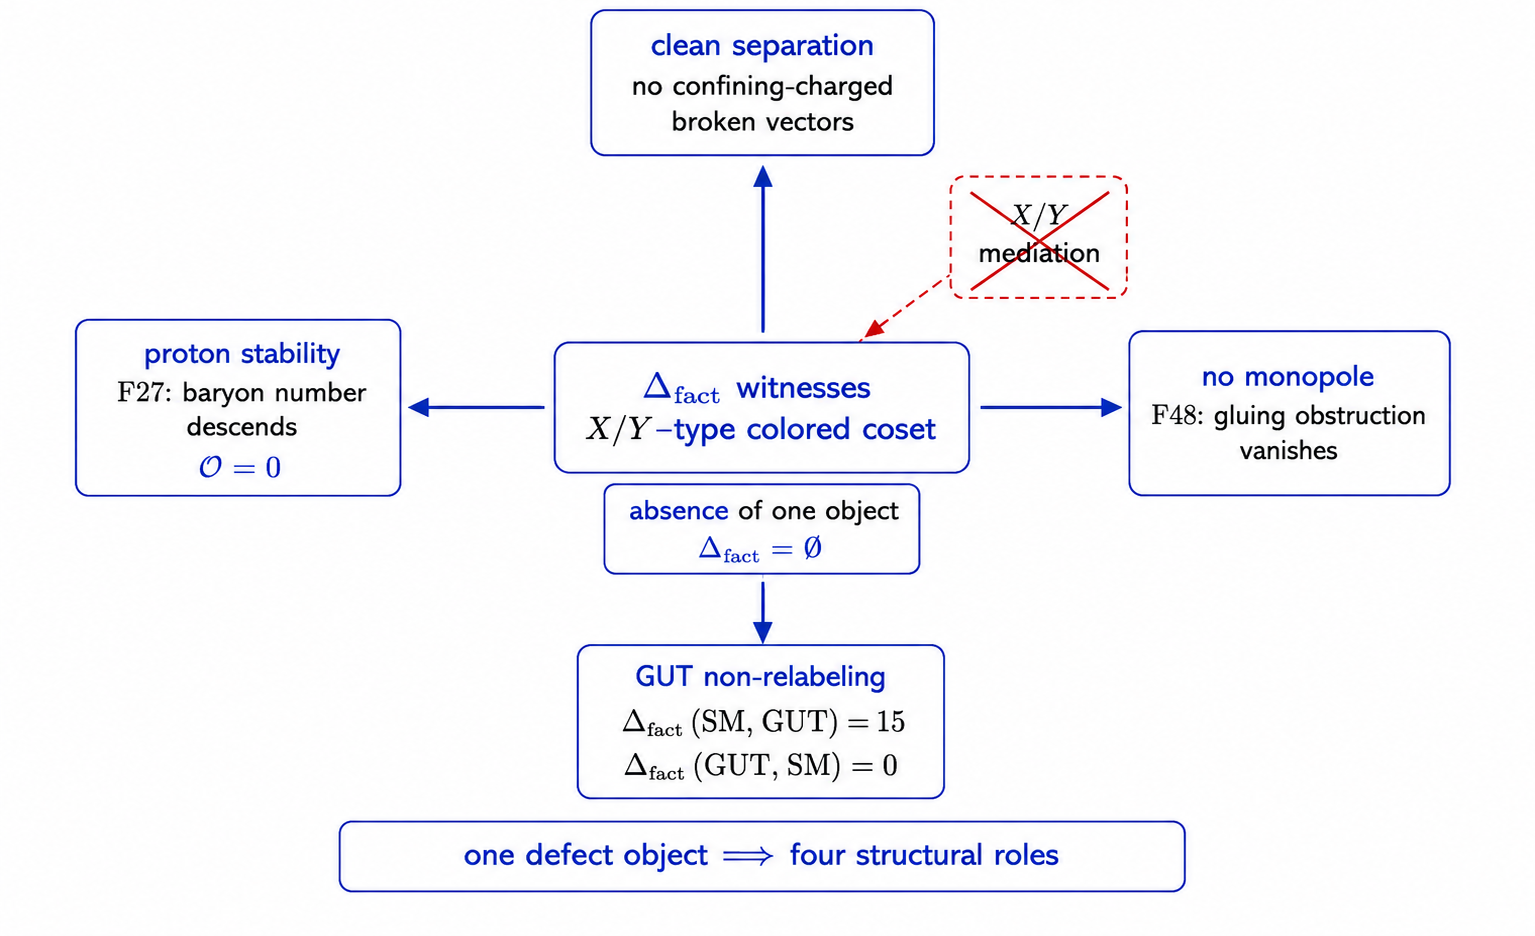
\includegraphics[width=0.7\linewidth]{figures/fig_f2_xy_coset_spine.png}
  \caption{\textbf{\(X/Y\)-coset spine.} \emph{One central node (\(\Delta_{\mathrm{fact}}\) witnesses) with four arrows --- clean-separation, proton stability (F27), no monopole (F48), GUT non-relabeling --- annotated ``absence of one object \(\Rightarrow\) all four at once.''}}
  \label{fig:f2}
\end{figure}

Constructing the F51 common-refinement parent over the SM's two routes lands the embedding numbers \textbf{as computations,
not inputs}. Over one SM generation,

\[
\sin^2\theta_W \;=\; \frac{\operatorname{Tr} T_3^2}{\operatorname{Tr} Q^2}
\;=\; \frac{2}{16/3} \;=\; \frac{3}{8},
\qquad
k_Y \;=\; \frac{5}{3} \ \ \text{(from } \operatorname{Tr} Y^2 = \tfrac{5}{6}\text{)} ,
\]

with the traces computed from the SM charge table (declared input) and the \emph{minimal-simple} parent class (declared
source). Non-circularity has a computed control: a product parent satisfying the same bare requirement yields \(3/23\),
so the value \(3/8\) genuinely depends on the declared source rather than being baked in (\textbf{GROUND}, conditional on that
source). Scope is strict: these are the \emph{embedding} ratios; the measured low-energy \(\sin^2\theta_W\) requires
renormalization-group running to a physical scale, which the toy does not contain --- and the flagship unification test
\textbf{fails} for minimal non-supersymmetric \(SU(5)\)~\citep{GeorgiGlashow1974}, consistent with experiment~\citep{SuperK2020}.

\hypertarget{grounding-the-condition-record-stability}{%
\subsection{Grounding the condition: record-stability}\label{grounding-the-condition-record-stability}}

Clean separation itself is not toy-derivable (the only internal grounding is circular --- caught and rejected). It is
\textbf{grounded one layer up} (\textbf{GROUND}): requiring a \emph{memory/record-stability} layer --- a stable confining substrate, the
capacity for at least two neutral records, and distinguishability --- \textbf{forces} clean separation. On the full carrier:

\[
\#\{\,\text{record-stable} \wedge \Delta_{\mathrm{fact}}\neq\varnothing\,\} \;=\; 0
\quad\text{out of } 11{,}990 .
\]

Anti-circularity is computed, not asserted: the substrate conjunct alone admits \(60\) decaying structures, the capacity
conjunct alone admits \(311\); only the conjunction lands in the clean class, and record-stability is \emph{not} extensionally
clean-separation (\(24\) record-stable structures versus \(316\) clean --- a strict directional implication). The
all-structures theorem upgrade (lemma L60\(\to\)L64) remains open and is tracked as such.

\hypertarget{the-blindness-theorems-what-is-proved-observed-input}{%
\subsection{\texorpdfstring{The blindness theorems: what is \emph{proved} observed-input}{The blindness theorems: what is proved observed-input}}\label{the-blindness-theorems-what-is-proved-observed-input}}

The demarcation's other half is proof-grade negatives (\textbf{PROVE-BLIND}):

\begin{itemize}
\tightlist
\item
  \textbf{Generation count.} For an anomaly-free content unit with an even per-unit \(SU(2)\)-doublet count (the SM unit
  qualifies), every gate of the frozen closure chain is invariant in \(N_{\mathrm{gen}}\): anomaly coefficients scale
  linearly (\(N\cdot u\)), the Witten parity gate~\citep{Witten1982} depends only on \((N\cdot d)\bmod 2\), and the remaining gates are
  nonempty-gated. Hence the chain passes identically for \textbf{all} \(N \ge 1\) (constructed theorem; an odd-doublet control
  \emph{is} \(N\)-sensitive, so the hypothesis is load-bearing). The calculus cannot see \(N_{\mathrm{gen}}=3\); the only handle
  is the recognition-source bound \((N-1)(N-2)/2 > 0 \iff N \ge 3\) from CP violation~\citep{KobayashiMaskawa1973} --- observed-input.
\item
  \textbf{Content.} Within the selected gauge structure, three definitionally distinct neutral shadows (integer charge
  quantization of the color-singlet spectrum; Yukawa-texture connectivity; mass-matrix rank) are all blind to the
  SM-vs-alternative content classes: the detailed matter content is a contingency-class residual (F26).
\item
  \textbf{Scales and values.} The electroweak scale is reframed (not solved) as an F47 small-selector region (\(\approx 3.96\%\)); no measured low-energy observable is derived anywhere in the track.
\end{itemize}

\hypertarget{result-sm-summary-table}{%
\subsection{Summary table}\label{result-sm-summary-table}}

\begin{longtable}[]{@{}lll@{}}
\toprule
\begin{minipage}[b]{0.28\columnwidth}\raggedright
question\strut
\end{minipage} & \begin{minipage}[b]{0.31\columnwidth}\raggedright
verdict (grade)\strut
\end{minipage} & \begin{minipage}[b]{0.34\columnwidth}\raggedright
basis\strut
\end{minipage}\tabularnewline
\midrule
\endhead
\begin{minipage}[t]{0.28\columnwidth}\raggedright
exclude \(\sim99.3\%\) of chiral gauge structures\strut
\end{minipage} & \begin{minipage}[t]{0.31\columnwidth}\raggedright
\textbf{COMPUTE}, unconditional\strut
\end{minipage} & \begin{minipage}[t]{0.34\columnwidth}\raggedright
closure chain on \(11{,}990\) structures\strut
\end{minipage}\tabularnewline
\begin{minipage}[t]{0.28\columnwidth}\raggedright
select \(\mathfrak{su}(2)\oplus\mathfrak{su}(3)\oplus\mathfrak{u}(1)\)\strut
\end{minipage} & \begin{minipage}[t]{0.31\columnwidth}\raggedright
\textbf{SELECT}, on clean separation\strut
\end{minipage} & \begin{minipage}[t]{0.34\columnwidth}\raggedright
\(\Delta_{\mathrm{fact}}=\varnothing\)\strut
\end{minipage}\tabularnewline
\begin{minipage}[t]{0.28\columnwidth}\raggedright
proton stability \(+\) no monopole \(+\) color separation\strut
\end{minipage} & \begin{minipage}[t]{0.31\columnwidth}\raggedright
\textbf{COMPUTE}\strut
\end{minipage} & \begin{minipage}[t]{0.34\columnwidth}\raggedright
one object: the \(X/Y\) coset, absent\strut
\end{minipage}\tabularnewline
\begin{minipage}[t]{0.28\columnwidth}\raggedright
\(\sin^2\theta_W = 3/8\), \(k_Y = 5/3\)\strut
\end{minipage} & \begin{minipage}[t]{0.31\columnwidth}\raggedright
\textbf{GROUND} (minimal-simple parent)\strut
\end{minipage} & \begin{minipage}[t]{0.34\columnwidth}\raggedright
trace ratios; product control \(3/23\)\strut
\end{minipage}\tabularnewline
\begin{minipage}[t]{0.28\columnwidth}\raggedright
clean separation itself\strut
\end{minipage} & \begin{minipage}[t]{0.31\columnwidth}\raggedright
\textbf{GROUND} (record-stability)\strut
\end{minipage} & \begin{minipage}[t]{0.34\columnwidth}\raggedright
\(0/11{,}990\) counterexamples; non-circular\strut
\end{minipage}\tabularnewline
\begin{minipage}[t]{0.28\columnwidth}\raggedright
single-factor exclusion, all \(N\)\strut
\end{minipage} & \begin{minipage}[t]{0.31\columnwidth}\raggedright
\textbf{COMPUTE} (constructed theorem)\strut
\end{minipage} & \begin{minipage}[t]{0.34\columnwidth}\raggedright
symbolic proof\strut
\end{minipage}\tabularnewline
\begin{minipage}[t]{0.28\columnwidth}\raggedright
\(N_{\mathrm{gen}}\), content, measured values\strut
\end{minipage} & \begin{minipage}[t]{0.31\columnwidth}\raggedright
\textbf{PROVE-BLIND} / observed-input\strut
\end{minipage} & \begin{minipage}[t]{0.34\columnwidth}\raggedright
all-\(N\) theorem; three blind shadows\strut
\end{minipage}\tabularnewline
\begin{minipage}[t]{0.28\columnwidth}\raggedright
measured \(\sin^2\theta_W\), couplings, masses, EW scale\strut
\end{minipage} & \begin{minipage}[t]{0.31\columnwidth}\raggedright
\textbf{not landed} (out of scope)\strut
\end{minipage} & \begin{minipage}[t]{0.34\columnwidth}\raggedright
need running/scale = experiment\strut
\end{minipage}\tabularnewline
\bottomrule
\end{longtable}

The Standard Model, on this evidence, is not one derivable object. It is a \emph{selection} with a thin forced skeleton ---
and the calculus proves both the skeleton and the thinness. Section 6.3 turns the spine of this analysis into a
falsifiable prediction.

\hypertarget{result-ii-quantum-mechanics-general-relativity-as-a-common-refinement-a-unification}{%
\section{Result II --- conditional QM--GR access structures and graph duality}\label{result-ii-quantum-mechanics-general-relativity-as-a-common-refinement-a-unification}}

\hypertarget{locating-the-obstruction-the-route-mismatch}{%
\subsection{Route mismatch: an exact commutation result}\label{locating-the-obstruction-the-route-mismatch}}

For idempotent endomorphisms \(E_1,E_2\), the finite defect
\[
\Delta_3^{\mathrm{comp}}(E_1,E_2)=\{c:E_1E_2(c)\ne E_2E_1(c)\}
\]
is a legitimate mathematical measure of non-commutation, and non-commuting examples exist. The natural QM--GR
instantiation, however, gives a null verdict. On the 16-state Boolean carrier, the two conditional-mean completions are
idempotent and \textbf{commute exactly}: \(E_{\rm QM}E_{\rm GR}=E_{\rm GR}E_{\rm QM}\), so the defect set is empty. A
naive normalized distance between the two encoded tables (\(0.5\); \(1/\sqrt2\) under \(0/1\to\pm1\) recoding) is
encoding-dependent and is not a conjugacy-invariant commutator magnitude.

Coordinate conditional means commute here because the Boolean-cube overlap factorizes. Non-commuting idempotent pairs
can be constructed from non-factorizing partitions and constrained projections as mathematical controls,
but none is derived from the frozen ``quantize'' and ``curve'' routes. No route-mismatch explanation of why
quantizing gravity fails is therefore available at this level. Exact matrices and recoding controls are in
\nolinkurl{review_2026/repairs/q2_route_mismatch/}.

\hypertarget{the-resolution-a-fork-not-a-ladder}{%
\subsection{Fork-over-ladder, with finite provenance}\label{the-resolution-a-fork-not-a-ladder}}

A separate access-factorization result holds, narrowly. On the abstract four-coordinate carrier
\[
q_{\rm QM}=(d_0,d_1,d_2),\qquad q_{\rm GR}=(d_0,d_2,d_3),\qquad L=(d_0,d_1,d_2,d_3),
\]
\(q_{\rm GR}\) is not a deterministic quotient of \(q_{\rm QM}\): the two directed defects each have eight witnesses.
The nested coordinate control factors, while both readouts factor through \(L\) by definition. Exhausting all 16
coordinate-subset partitions gives 55 incomparable pairs among the 120 unordered distinct pairs. This is an exact toy
theorem conditional on the abstract carrier and its access interpretation; it is consistent with, and does not
contradict, the exact commutation of §5.1.

A finite provenance construction replaces bare mode labels. On 54
constructed \((\psi,V_0)\) records, coarse field functionals and explicit phase-only and potential controls realize
mutually non-factorizing QM and GR readouts. Its conditions are material: the forward witness changes \(V_0\), the QM
audit includes density and current rather than Born density alone, \(d_0\) is constant, and the realized coordinate
image is \(1\times2\times8\times3\), not the full \(2^4\) carrier. Nine hand-instantiated F24 representatives were
tested; two reconcile but are partition-equivalent to \(L\). Thus this is \textbf{conditional finite provenance}, not
family, type, or instance uniqueness. See \nolinkurl{review_2026/repairs/q1_access_provenance/}.

The theorem named \(T_{\mathrm{QG\text{-}NoGo}}\) is narrow: it tests two special fused or
stapled routes and does not quantify over general fused objects, coherent mediators, or operator algebras. It cannot
support any statement that quantum gravity is ``illegal'' in the grammar.

\begin{figure}[tbp]
  \centering
  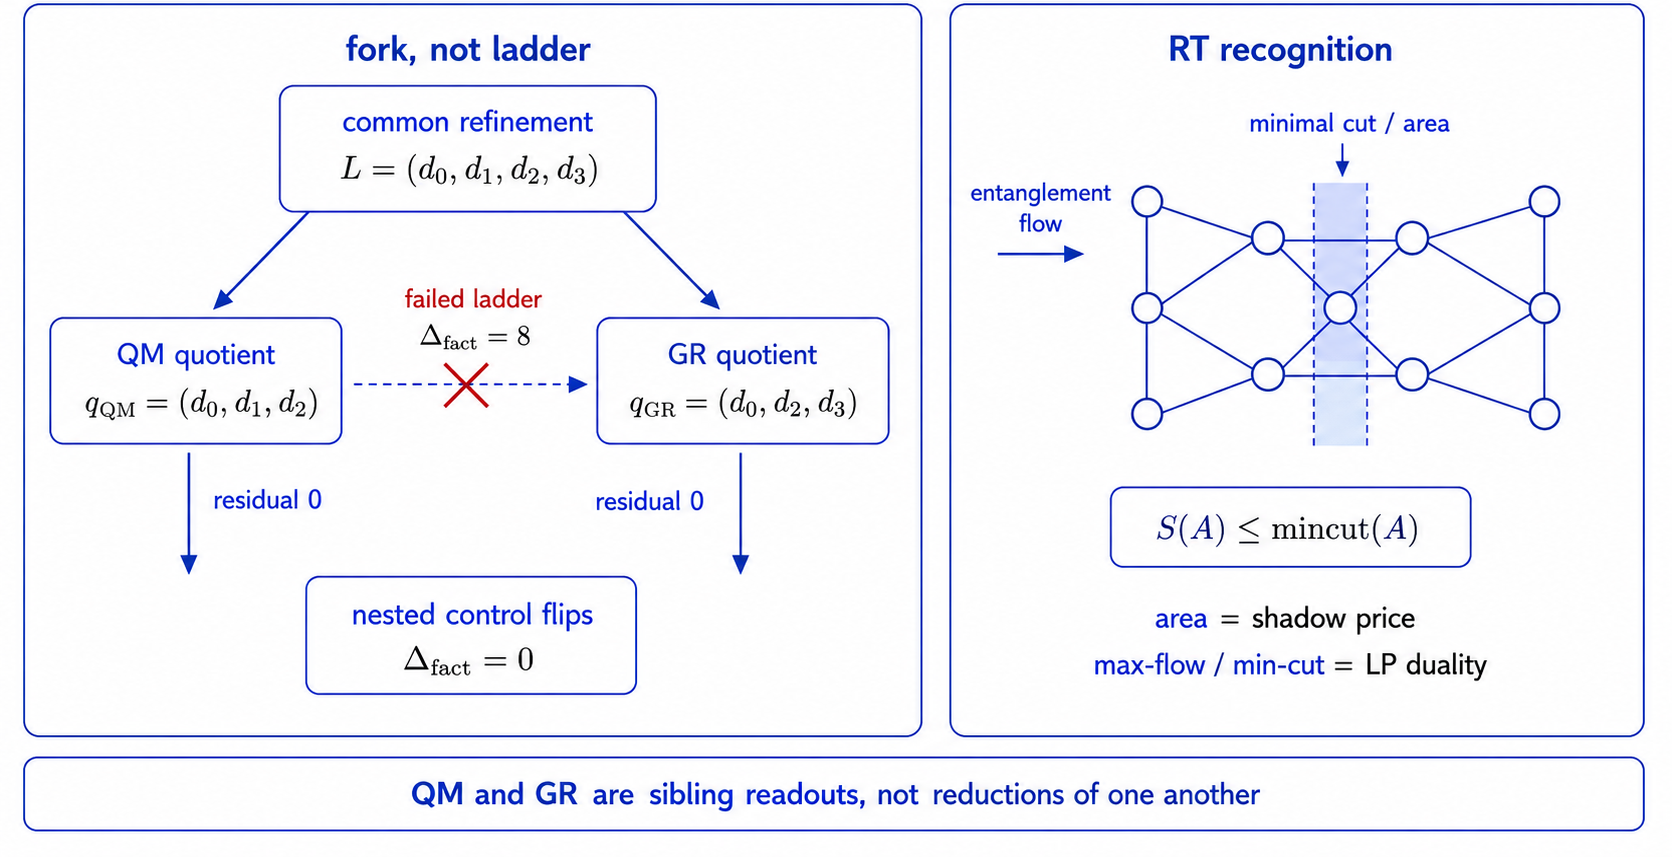
\includegraphics[width=\linewidth]{figures/fig_f3_fork_rt.png}
  \caption{\textbf{Finite fork and graph-duality constructions.} Left: the declared abstract access fork, for which the
  directed quotient fails and the common refinement closes. Right: a boundary-anchored flow network; the
  identity distinguishes the dual optimum from its per-edge shadow prices.}
  \label{fig:f3}
\end{figure}

\hypertarget{grounding-the-premise}{%
\subsection{The common carrier is a hypothesis}\label{grounding-the-premise}}

The common-carrier premise is not computationally grounded by the available tests. Semiclassical co-sourcing---one field
\(\psi\) supplying a Born-type readout and stress-energy for a potential---is a plausible named recognition source,
but the existing controls test different predicates and the ``door test'' is prose. The premise is therefore
carried as a declared hypothesis, not a GROUND landing. The 54-record construction above shows that a finite realization can
be built under explicit choices; it does not establish that nature, the free gravitational sector, or a deep
quantum-gravity regime shares such a carrier.

\hypertarget{recognition-ryutakayanagi-as-ledgershadow-price-duality}{%
\subsection{Finite-graph min-cut/LP-duality recognition}\label{recognition-ryutakayanagi-as-ledgershadow-price-duality}}

At nondegenerate seeded capacities, every tested
boundary region has a unique minimum cut with an exported margin. The max-flow primal and cut dual are exported as
matrices, and exact certificates verify strong duality and complementary slackness. If \(y_e\) denotes the dual
variable associated with edge capacity \(c_e\), then the identity is
\[
\operatorname{Area}(\operatorname{mincut}A)
=\operatorname{OPT}_{\rm dual}(A)
=\sum_e c_e y_e,
\]
where the \(y_e\)---not the dual optimum---are per-edge shadow prices. In the unique-cut chamber they are the \(0/1\)
cut-incidence variables and satisfy \(y_e=\partial F^*/\partial c_e\), verified by two-sided perturbations.

Independently contracted random-tensor states obey \(S(A)\le\operatorname{mincut}(A)\) on the sampled carrier. The ratios
\(S/\operatorname{mincut}=0.729,0.904,0.941\) for bond dimensions \(D=2,3,4\) are a \emph{finite sampled saturation
trend}, not convergence or equality; sampled contracted-state entropies remain below the cuts. The min-cut entropy
vectors satisfy monogamy, and a fairly compared GHZ control violates it. These results support a
\textbf{finite-graph recognition} of RT-related structure, conditional on the graph/tensor-network model; they do not
derive holography~\citep{RyuTakayanagi2006,Maldacena1998}, \(1/4G\), or a continuum law.

Two natural extensions fail, and the failures are results in their own right. First, there is no linearized-Einstein
match: a pass can be manufactured at a degenerate point, but
at an honest nondegenerate base point an independently specified geometry deformation does not match the
contracted-state \(\delta S\) under the declared pairing; uniqueness margins and a can-fail deformation are exported.
Second, Born and area do not carry one universal composition law: area follows min-plus composition on all four tested
gluing probes, while Born fails all four. The cross-ledger statement is only that the two sampled ledgers
obey the same monogamy inequality class, with different dependencies. See
\nolinkurl{review_2026/repairs/q5_lp_duality/}.

\hypertarget{result-qmgr-summary-table}{%
\subsection{Certified summary}\label{result-qmgr-summary-table}}

\begin{longtable}[]{@{}p{0.28\linewidth}p{0.22\linewidth}p{0.42\linewidth}@{}}
\toprule
question & status & certified scope\\
\midrule
\endhead
route mismatch & exact null result & completions commute; \(0.5\) is encoding-dependent table distance\\
fork-over-ladder & narrow exact theorem & exact coordinate-partition non-factorization on the declared Boolean carrier\\
field provenance & conditional finite construction & 54 records with named coarse functionals and stated limitations\\
common-carrier premise & hypothesis & semiclassical co-sourcing is a named physical motivation, not a landing\\
\(T_{\mathrm{QG\text{-}NoGo}}\) & narrow & two special fused/stapled routes only\\
RT/LP relation & finite-graph recognition & exact dual certificate and sensitivities on finite nondegenerate graph cuts\\
linearized Einstein & negative result & tested response does not match under the declared deformation pairing\\
one Born--area ledger & negative result & area passes four min-plus gluings; Born fails all four\\
\bottomrule
\end{longtable}

\hypertarget{open-programs-from-the-three-published-predictions}{%
\section{Construction programs from the three published predictions}\label{open-programs-from-the-three-published-predictions}}

Version 1 presented three predictions as forced and falsifiable. Post-publication verification showed that none was forced by
the published machinery. This section retracts that headline and separates reproducible finite statements from three
construction programs, the first now resolved within declared scope. Falsifiability language is retained only for a
specified finite model or conditional
channel; it is not transferred to nature where the required bridge has not been built.

\hypertarget{the-entanglement-geometry-question-open-program}{%
\subsection{The entanglement--geometry question (resolved within declared scope)}\label{the-entanglement-geometry-question-open-program}}

The published carrier had fourteen edge capacities: eight terminal leaves and three bivalent two-edge bridges. Its
11,049-component min-cut fingerprint had raw Jacobian rank nine and nullity five. Exact series/parallel reduction shows
that all six bridge capacities enter only through
\[
K=\sum_{i=1}^{3}\min(w_{LM_i},w_{M_iR}).
\]
The nine effective coordinates---eight leaves and \(K\)---have rank nine and nullity zero on all three published seeds.
Thus the published kernel is parameterization redundancy, not evidence that physically distinct geometries share one
fingerprint.

The repaired graph probe replaces finite differences by the exact active-cut incidence matrix. For each boundary region
it enumerates the unique minimizing cut, records its margin, and computes rational rank. Five exact local reduction
classes are then applied: saturated-terminal/zero-column contraction; inseparable-vertex contraction with parallel sums;
series reduction; exact two-terminal module replacement; and exact \(\Delta\)--Y/Y--\(\Delta\) replacement. The fifth
move is accepted only when complete re-enumeration preserves every rational boundary cut value and continued uniqueness.

Within 378 weighted carriers and the declared \textbf{three-round} \(\Delta\)--Y/Y--\(\Delta\) presentation search,
365 reduce to full rank. Thirteen remain, with residual-deficiency histogram
\[
1^8,\qquad 2^4,\qquad 3^1.
\]
The named \(K_{2,3}\) carrier retains a one-dimensional kernel after the five classes; all 62 cut values and unique
minimizers survive its accepted moves. Two equal-coefficient candidate sixth directions---a \(K_{2,3}\) four-cycle
transportation redistribution and a \(K_4\) opposite-perfect-matching redistribution---explain none of the selected
thirteen survivors. This does \emph{not} prove irreducibility: exact graph quotients are not exhausted, and the two
sixth-move ansätze are only diagnostics. Artifacts and the byte-comparing validator are in
\nolinkurl{review_2026/probes/p1_kernel_quotient/}.

The finite census is directly falsifiable by re-enumeration: a different rank, cut value, uniqueness result, or named
reduction path would refute it. The former physical prediction is not established. Version 2 left two open routes;
both were executed after publication of Version 2, with reviewer-certified artifacts and byte-comparing validators
under \nolinkurl{open_programs/} in the repository.

\emph{Route 1 (graph level) --- resolved within the declared five-class relation.} The local-move repertoire is
provably complete at the star-mesh level: no local \(k\)-star-mesh transform preserves min-cut for \(k>3\)
(Kalman--Krauthgamer, arXiv:2112.06916, Thm.~3.24), so the five declared classes are not an arbitrary stopping point.
Exact-rational recertification confirms all thirteen residual carriers (the three near-float-tolerance minimum margins
are strictly positive; no earlier carrier classification changed). Every carrier admits at least one nondegenerate exact rational
weight interval of same-graph fibers: nineteen kernel-basis directions in all, each yielding distinct positive
weightings with identical complete terminal min-cut fingerprints, re-established by exhaustive enumeration, with no
graph automorphism relating the endpoints. The two endpoint orbits of every fiber are disjoint after complete
queue-exhaustive closure under the five declared exact fingerprint-preserving move classes, modulo terminal-label-fixed
exact weighted isomorphism; all nonidentity admitted transitions are \(\Delta\)--Y/Y--\(\Delta\). Transformations
outside the declared classes remain open.

\emph{Route 2 (state level) --- resolved within declared scope: six exact examples.} An explicit dense-numerical
contracted-state entropy engine, with verified tensor-presentation moves and non-vacuous controls, first shows the
preregistered convention-scoped negative: under the initial declared injective capacity-to-state convention, all nineteen cut-fiber pairs
split at the state level, and across a preregistered five-member convention/tensor family every seeded-random row has
trivial cut/state-kernel intersection. The connected-copy member \(C2\_L1\), however, carries six analytically symmetry-protected
directions (its boundary state depends on capacities only through their product). Searching the complete cut kernel
constructs six positive exact-algebraic finite continuations with identical complete cut fingerprints, exactly equal
capacity products, and identical connected-copy boundary states. Under the frozen family gauge relation ---
terminal-fixed weighted isomorphism, tensor-presentation gauge not acting on capacities, boundary-local unitaries, and
identity or global all-edge reciprocal as the only family-returning reciprocal actions --- all six pairs are exact
finite declared-gauge underdetermination examples, separated by the exact invariant
\(I(c)=\{\sum_e c_e,\ \sum_e c_e^{-1}\}\). Cut-preserving \(\Delta\)--Y moves are excluded from the state-gauge
relation by an exact countercheck (an admitted move preserves every cut value while changing the copy product). This
conclusion is specific to these finite carriers, the connected-copy tensor family, the declared capacity convention,
and the frozen gauge relation; other tensor families and conventions, broader physical gauge relations, continuum
limits, and any interpretation as underdetermination of bulk geometry remain open.

\hypertarget{bmv-conditional-statement}{%
\subsection{BMV (conditional statement)}\label{bmv-conditional-statement}}

The finite quantum-information calculation is correct under its explicit premise. If the gravitational mediator is
assumed to be a perfect classical-record channel---measure a geometry-visible label, store it in orthogonal records,
and condition local responses only on that label---then the induced two-mass channel is LOCC. Exact density-matrix
calculation gives zero negativity and no CHSH violation, while a coherent-control channel entangles. This is a standard
conditional consequence of the assumed channel.

What fails is the forcing step. The access tuple and narrow fused-route no-go do not derive a record channel. A
geometry-diagonal coherent countermodel preserves the declared visible information while retaining phase coherence, and
the historical ``mean-field guard'' was only a six-token source grep. Therefore the claimed prohibition on
gravitationally mediated entanglement and the corresponding BMV-null forcing~\citep{Bose2017,MarlettoVedral2017}
are retracted.

Within the assumed perfect-record model, a nonzero entanglement output would falsify the implementation or the channel
assumption. A positive physical BMV observation would rule out that channel as a model of the experiment, but would not
falsify a derivation that this paper does not possess. The open task is dynamical: derive, or fail to derive, record
formation and decoherence from an explicit gravitational interaction without stipulating orthogonal records.

\hypertarget{record-stability-open-program}{%
\subsection{Record stability (open program)}\label{record-stability-open-program}}

The published implication from record stability to absence of proton-decay and monopole mediators had two successive
problems. Its original table treated \(\Delta_{\mathrm{fact}}\)-undefined rows as breaking. A full-carrier repair evaluated
the defect wherever confinement made it defined and recovered a conditional implication under a restricted record-token
grammar. But branch-complete ablations then showed that the implication changes when the token census changes.

The most inclusive certified probe enumerates residual-invariant candidate operators within a declared bound: fermion
arity \(2\) through \(4\), enough to cover the largest residual epsilon arity plus one; scalar or VEV dressings
\(\phi,\phi^\dagger\) up to two insertions; and at most six total constituents. It requires exact singlet multiplicity
under every unbroken residual factor and neutrality under the scalar-stabilizer-derived residual \(U(1)\). In particular,
the regression operator \(\epsilon(o_{2c0},o_{3c0})\), with UV lift
\(\epsilon\,o_2o_3\phi^\dagger\) and charges \(-2+4-2=0\), must be counted; the earlier spectator-Cartan token must not.

With scalar-dressed candidates admitted uniformly on clean and breaking branches, all three readings---pointwise
\(RS(C,\phi)\Rightarrow\mathrm{Clean}(C,\phi)\), structure-universal, and structure-existential---have counterexamples
at the declared thresholds. Excluding dressed candidates can restore the implication, so the result is
\textbf{token-definition-sensitive}. The enumerated monomials are not physical-state counts: no Grassmann/EOM/syzygy
quotient and no UV-to-residual restriction rank was computed. See
\nolinkurl{review_2026/repairs/s6_record_grammar_ablation/}.

Consequently, no result here presently excludes proton decay or monopoles, and an observation of either is not
a falsifier of a theorem established here. The sharply posed open program is to define records dynamically and test
which invariant candidates persist under the branch's actual evolution. Only such a persistence criterion could turn
the algebraic census into a physical statement.

\hypertarget{prediction-status-summary}{%
\subsection{Status summary}\label{prediction-status-summary}}

\begin{longtable}[]{@{}p{0.20\linewidth}p{0.20\linewidth}p{0.52\linewidth}@{}}
\toprule
former prediction & Version-3 status & surviving statement\\
\midrule
\endhead
entanglement \(\ne\) geometry & resolved within declared finite scope & 19 exact same-graph fibers have disjoint complete
orbits under the five declared move classes modulo terminal-label-fixed exact weighted isomorphism; six exact finite
\(C2\_L1\) examples survive the declared convention and frozen family gauge; undeclared transformations and bulk-geometry
interpretation remain open\\
BMV-null & forcing retracted & perfect-record channel is LOCC and BMV-null; derivation of that channel is open\\
record-stability forcing & forcing retracted & bounded candidate census is token-definition-sensitive;
dynamical record persistence is open\\
\bottomrule
\end{longtable}

\hypertarget{breadth-one-calculus-three-more-deep-problems}{%
\section{Breadth: one calculus, three more deep problems}\label{breadth-one-calculus-three-more-deep-problems}}

The universality thesis (§8) gains most of its force from breadth: the \emph{same} obstruction/defect/moduli machinery that
produced Sections 4--6, applied without modification, classifies three further foundational puzzles. Each result below
is a computed forbidden-rule or demarcation with its own can-fail control. None is new physics --- each recovers or
classifies known structure --- and that is their role: they show the grammar is one object, not a per-problem retrofit.

\hypertarget{bell-nonlocality-the-common-carrier-is-not-a-hidden-variable}{%
\subsection{Bell nonlocality: the common carrier is not a hidden variable}\label{bell-nonlocality-the-common-carrier-is-not-a-hidden-variable}}

The common-carrier premise of §5.3 invites an immediate objection: a single carrier \(\psi\) underlying both readouts
\emph{sounds like} a local hidden variable --- and local hidden variables are experimentally dead. The calculus's F49 normal
form turns the objection into a computation. For a Bell pair with standard CHSH settings~\citep{Bell1964,CHSH1969} (\(a_0 = Z\), \(a_1 = X\),
\(b_{0,1} = (Z \pm X)/\sqrt2\)), the correlation table is computed from the state, giving

\[
\mathrm{CHSH}_{\mathrm{quantum}} = 2\sqrt2 \approx 2.8284 ,
\]

while the local bound is \textbf{enumerated} --- all \(16\) deterministic local strategies, \(\max = 2\) exactly. The F49
common-source test (does any setting-independent source quotient factor both readouts?) therefore fails --- the
correlation is a \emph{statused nonlocal residual}, Bell's theorem recovered as a normal form. The can-fail control
discriminates: a classical mixture (\(\mathrm{CHSH} = \sqrt2\)) \textbf{is} locally explainable, with an explicit 16-row
hidden-variable table reproducing its correlations to \(1.8\times10^{-15}\).

The calculus-specific content is the reconciliation: F49's ``common source'' must be an \emph{admissible access quotient}, and F37
(complementarity as non-joint-access) forecloses exactly that for the non-commuting settings --- the computed setting
commutators (\(0.707\)) coincide with the carrier's complementary-pair control. The carrier lives \textbf{above} the access
structure; it is not, and cannot be, a local hidden variable. \textbf{Forbidden rule:} \emph{any reading of a common-carrier
framework in which the carrier functions as a local hidden variable is excluded} --- the premise survives Bell precisely
because the joint quotient it would require does not exist.

\hypertarget{black-hole-information-loss-is-a-property-of-the-readout-not-the-carrier}{%
\subsection{Black-hole information: loss is a property of the readout, not the carrier}\label{black-hole-information-loss-is-a-property-of-the-readout-not-the-carrier}}

The F34 information-loss normal form asks of any transport \(\tau: H_0 \to H_1\) with recovery readout \(\rho\) and source
information \(\sigma\): is the obstruction set

\[
\mathcal O_\rho \;=\; \{(h,h') : \rho(\tau h) = \rho(\tau h') \ \wedge\ \sigma(h) \neq \sigma(h')\}
\]

empty (recoverable) or not (loss)? Instantiated on the holographic carrier with \(\tau\) the bulk\(\to\)boundary
contraction, the verdict is exact and two-sided. The preimage classes of the full boundary state are \textbf{precisely the
internal gauge orbits}: \(\operatorname{rank} = 27\) = internal dimension (computed), and for any two preimages an
explicit gauge transformation \(G\) connecting them is solved for and verified (residual \(3\times10^{-15}\)). Hence at the
\textbf{full boundary}, the only lost interior data is gauge --- every gauge-invariant (physical) interior observable is
recoverable: loss is \emph{F34-legitimate}. At a \textbf{partial readout} (the reduced state on half the boundary --- the
``early radiation only'' analog), loss is real: an exact witness applies a unitary on the unobserved half, leaving the
observed reduced state identical (\(5\times10^{-16}\)) while gauge-invariant physical observables shift (\(\approx 10^{-2}\)). \textbf{Forbidden rule:} \emph{the holographic carrier forbids physical-information loss at the full-boundary
recovery; loss is forced at partial/coarse readouts} --- in this toy, the information paradox~\citep{Hawking1976} is a property of the
readout, not of the carrier. (No dynamics, no evaporation, no Page curve~\citep{Page1993} is claimed.)

\hypertarget{the-cosmological-constant-no-in-layer-value-law}{%
\subsection{The cosmological constant: no in-layer value-law}\label{the-cosmological-constant-no-in-layer-value-law}}

The F50 vacuum/background-selection law classifies a background quantity as \textbf{necessary} (closure fixes one value),
\textbf{moduli} (closure is blind --- contingent), or \textbf{vacuum-selected} (a singleton selector). The carrier of §5.3 contains
the cosmological-constant analog~\citep{Weinberg1989} explicitly: the matter-independent background term in \(V[\psi] = V_0 + \kappa\, T_{00}[\psi]\). Sweeping it through the frozen closure chain: \(15\) of \(18\) background values pass (degeneracy \(15\), no
singleton selector; the pass set is bounded and non-contiguous), so the background is \textbf{F50 bounded-moduli} --- the
closure does not select its value. The discrimination control is the coupling \(\kappa\), which the same chain \emph{does}
constrain (a computed admissibility boundary: \(\kappa \le 10\) converges, \(\kappa \ge 15\) runs away) --- so the audit
distinguishes closure-constrained parameters from genuine moduli; it is not an everything-is-contingent verdict.
\textbf{Demarcation:} \emph{no in-layer \(\Lambda\) value-law exists; any claimed in-layer derivation of \(\Lambda\)'s value must
smuggle a selection; the in-layer content is at most an admissibility window.} This is the same F47/F26 demarcation
pattern the SM track exhibits for its contingent quantities --- the cross-track recurrence is itself evidence for §8.

\hypertarget{the-measurement-problem-a-structural-discriminator}{%
\subsection{The measurement problem: a structural discriminator}\label{the-measurement-problem-a-structural-discriminator}}

(From the SM-track extension; included for completeness of the breadth claim.) Measurement-selection --- ``which outcome
becomes the fact'' --- is proven an \textbf{irreducible strict extension} of quantum mechanics in the calculus: records are
\(\Sigma_f\)-definable, selection is not, by an explicit non-factorization witness. The constructive payoff is a
\emph{no-fitting} discriminator: any future single-outcome theory must either modify the defect ledger \(D\)
(objective-collapse family) or only the readout \(\Sigma_f\) (many-worlds family); a community-accepted single-outcome
theory touching \emph{neither} would falsify the claim. This stakes a structural prediction about \emph{where any future theory
must land}, before such a theory exists.

\hypertarget{the-pattern}{%
\subsection{The pattern}\label{the-pattern}}

\begin{longtable}[]{@{}llll@{}}
\toprule
\begin{minipage}[b]{0.17\columnwidth}\raggedright
puzzle\strut
\end{minipage} & \begin{minipage}[b]{0.15\columnwidth}\raggedright
law\strut
\end{minipage} & \begin{minipage}[b]{0.32\columnwidth}\raggedright
verdict\strut
\end{minipage} & \begin{minipage}[b]{0.26\columnwidth}\raggedright
control\strut
\end{minipage}\tabularnewline
\midrule
\endhead
\begin{minipage}[t]{0.17\columnwidth}\raggedright
Bell nonlocality\strut
\end{minipage} & \begin{minipage}[t]{0.15\columnwidth}\raggedright
F49 + F37\strut
\end{minipage} & \begin{minipage}[t]{0.32\columnwidth}\raggedright
nonlocal residual recovered; carrier \(\neq\) hidden variable (forbidden rule)\strut
\end{minipage} & \begin{minipage}[t]{0.26\columnwidth}\raggedright
classical mixture: locally explainable, LHV table exhibited\strut
\end{minipage}\tabularnewline
\begin{minipage}[t]{0.17\columnwidth}\raggedright
BH information\strut
\end{minipage} & \begin{minipage}[t]{0.15\columnwidth}\raggedright
F34\strut
\end{minipage} & \begin{minipage}[t]{0.32\columnwidth}\raggedright
loss gauge-only at full boundary; real at partial readouts\strut
\end{minipage} & \begin{minipage}[t]{0.26\columnwidth}\raggedright
exact complement-unitary witness\strut
\end{minipage}\tabularnewline
\begin{minipage}[t]{0.17\columnwidth}\raggedright
cosmological constant\strut
\end{minipage} & \begin{minipage}[t]{0.15\columnwidth}\raggedright
F50 (+F47/F26)\strut
\end{minipage} & \begin{minipage}[t]{0.32\columnwidth}\raggedright
bounded-moduli; no in-layer value-law\strut
\end{minipage} & \begin{minipage}[t]{0.26\columnwidth}\raggedright
\(\kappa\): closure-constrained boundary\strut
\end{minipage}\tabularnewline
\begin{minipage}[t]{0.17\columnwidth}\raggedright
measurement\strut
\end{minipage} & \begin{minipage}[t]{0.15\columnwidth}\raggedright
non-factorization\strut
\end{minipage} & \begin{minipage}[t]{0.32\columnwidth}\raggedright
irreducible strict extension; \(D\)-vs-\(\Sigma_f\) discriminator\strut
\end{minipage} & \begin{minipage}[t]{0.26\columnwidth}\raggedright
identical-diagonal witness pair\strut
\end{minipage}\tabularnewline
\bottomrule
\end{longtable}

One grammar; six foundational puzzles (counting §6's three); every verdict computed, controlled, and graded.

\hypertarget{cross-track-ties-and-the-one-grammar-thesis}{%
\section{Cross-track ties, and the one-grammar thesis}\label{cross-track-ties-and-the-one-grammar-thesis}}

The per-track results stand on their own. But the calculus offers something that neither track shows alone and that, to
our knowledge, no other framework in either domain produces: \textbf{the same structural object turning out to be two
different physical phenomena}, on substrates that share no physics. These cross-track ties are not analogies or shared
tooling --- they are single objects in one grammar, read on two substrates that were explicitly guarded against each
other. We catalog them first (§8.2), argue why they are distinctive rather than coincidental (§8.3), and then draw the
thesis they support (§8.4).

\hypertarget{why-the-ties-are-non-trivial-the-anti-contamination-guard}{%
\subsection{Why the ties are non-trivial: the anti-contamination guard}\label{why-the-ties-are-non-trivial-the-anti-contamination-guard}}

The evidential weight of ``one object, two phenomena'' collapses if the two constructions were allowed to copy each
other. They were not. An \textbf{anti-contamination protocol} was declared at the outset: the SM substrate is a
\emph{selection/measure} layer (\(P_2\)-dominant --- a candidate space, constraints, a measure); the QM--GR substrate is a
\emph{co-sourcing common refinement} (\(P_4\)/F51 --- one field, two readouts). Build validators on the SM track fail on any
field-carrier token; steps that pattern-matched one substrate onto the other were rejected during construction
(Section 3.4). So when a single object surfaces on both tracks, it is because the \emph{law} is layer-agnostic --- not because
one construction borrowed from the other. Every tie below survived that guard.

\hypertarget{the-cross-track-ties}{%
\subsection{The cross-track ties}\label{the-cross-track-ties}}

\begin{quote}
\textbf{Each row is one object, computed on both substrates.} Read across: the leftmost column is a single construct of the
calculus; the next two columns are what it \emph{is} on each track.
\end{quote}

\begin{longtable}[]{@{}lll@{}}
\toprule
\begin{minipage}[b]{0.23\columnwidth}\raggedright
one calculus object\strut
\end{minipage} & \begin{minipage}[b]{0.35\columnwidth}\raggedright
on the SM substrate (selection layer)\strut
\end{minipage} & \begin{minipage}[b]{0.35\columnwidth}\raggedright
on the QM--GR substrate (common refinement)\strut
\end{minipage}\tabularnewline
\midrule
\endhead
\begin{minipage}[t]{0.23\columnwidth}\raggedright
\textbf{factorization defect} \(\Delta_{\mathrm{fact}}\)\strut
\end{minipage} & \begin{minipage}[t]{0.35\columnwidth}\raggedright
the \(X/Y\) colored coset --- proton decay, monopole, color-separation, GUT non-relabeling, one object (§4.4)\strut
\end{minipage} & \begin{minipage}[t]{0.35\columnwidth}\raggedright
the ladder defect (\(8\) witnesses) + the route-mismatch \(\Delta_3^{\mathrm{comp}}\) --- \emph{non-renormalizability} (§5.1--5.2)\strut
\end{minipage}\tabularnewline
\begin{minipage}[t]{0.23\columnwidth}\raggedright
\textbf{the record / memory rung}\strut
\end{minipage} & \begin{minipage}[t]{0.35\columnwidth}\raggedright
grounds clean-separation, \emph{forbids proton decay \& monopoles} (Pred. 3); hosts the measurement discriminator\strut
\end{minipage} & \begin{minipage}[t]{0.35\columnwidth}\raggedright
grounds the common carrier; makes the gravitational channel a record channel --- \emph{forbids BMV entanglement} (Pred. 2)\strut
\end{minipage}\tabularnewline
\begin{minipage}[t]{0.23\columnwidth}\raggedright
\textbf{F51 common refinement}\strut
\end{minipage} & \begin{minipage}[t]{0.35\columnwidth}\raggedright
the GUT parent → \(\sin^2\theta_W = 3/8\), \(k_Y = 5/3\) (trace ratios)\strut
\end{minipage} & \begin{minipage}[t]{0.35\columnwidth}\raggedright
the parent \(L\) → fork-over-ladder; forces the monogamy combiner\strut
\end{minipage}\tabularnewline
\begin{minipage}[t]{0.23\columnwidth}\raggedright
\textbf{GROUND landing mode}\strut
\end{minipage} & \begin{minipage}[t]{0.35\columnwidth}\raggedright
clean-separation \(\leftarrow\) record-stability\strut
\end{minipage} & \begin{minipage}[t]{0.35\columnwidth}\raggedright
common carrier \(\leftarrow\) semiclassical co-sourcing\strut
\end{minipage}\tabularnewline
\begin{minipage}[t]{0.23\columnwidth}\raggedright
\textbf{F37 complementarity} (non-joint-access)\strut
\end{minipage} & \begin{minipage}[t]{0.35\columnwidth}\raggedright
(the access-quotient discipline of the selection layer)\strut
\end{minipage} & \begin{minipage}[t]{0.35\columnwidth}\raggedright
the premise controls (no joint quotient for non-commuting accesses); reconciles the carrier with Bell (§7.1)\strut
\end{minipage}\tabularnewline
\begin{minipage}[t]{0.23\columnwidth}\raggedright
\textbf{F47/F26 demarcation} (no value-law on contingent selection)\strut
\end{minipage} & \begin{minipage}[t]{0.35\columnwidth}\raggedright
no value-law on the EW scale, \(N_{\mathrm{gen}}\), content\strut
\end{minipage} & \begin{minipage}[t]{0.35\columnwidth}\raggedright
no in-layer \(\Lambda\) value-law (F50 bounded-moduli, §7.3)\strut
\end{minipage}\tabularnewline
\bottomrule
\end{longtable}

Three of these are physical statements, not bookkeeping:

\begin{itemize}
\item
  \textbf{One defect is both proton physics and non-renormalizability.} \(\Delta_{\mathrm{fact}}\) --- the failure of one
  readout to factor through another --- is, on the SM substrate, the \(X/Y\) coset whose \emph{absence} makes the proton stable;
  on the QM--GR substrate, it is the obstruction that makes quantizing gravity fail. The calculus says these two
  century-old difficulties are the \emph{same kind of structural fact} about layered descriptions, surfacing on different
  substrates.
\item
  \textbf{One rung underlies three of the paper's headline results.} Record/memory stability --- the requirement that a
  universe be able to hold stable records --- grounds the SM gauge selection (§4.5), forbids proton decay (Prediction 3),
  \emph{and} forces the gravitational channel to be a record channel that decoheres without entangling (Prediction 2). A
  single structural commitment, stated once, has consequences in particle physics \emph{and} in tabletop gravity. This is
  the most consequential tie: it predicts that \emph{whatever forbids the proton from decaying is the same structure that
  prevents gravity from entangling masses} --- a connection no separate treatment of the two would suggest.
\item
  \textbf{One refinement law lands a gauge angle and resolves quantum gravity's architecture.} F51 (unification as common
  refinement) builds the GUT parent that yields \(\sin^2\theta_W = 3/8\) on one substrate and the QM--GR parent that
  selects the fork on the other --- the same commuting-square construction, two unrelated payoffs.
\end{itemize}

\hypertarget{why-this-is-distinctive-and-not-coincidence}{%
\subsection{Why this is distinctive --- and not coincidence}\label{why-this-is-distinctive-and-not-coincidence}}

Two reasons these ties are evidence rather than wordplay. First, \textbf{the anti-contamination guard} (§8.1): the objects
recur across substrates that were prevented from sharing structure, so the recurrence is forced by the laws. Second,
\textbf{the ties do work} --- each is load-bearing in a \emph{result}, not decorative: the shared record rung is what lets
Predictions 2 and 3 use one record constraint without collapsing their distinct physical claims; the shared \(\Delta_{\mathrm{fact}}\) is what lets the
non-renormalizability typing and the proton-stability spine be checked by one piece of frozen machinery. A coincidence
of notation could do neither.

This is, we contend, a distinctive feature of a layer-agnostic calculus, and one not easily reproduced by
domain-specific methods: a quantum-gravity framework has no reason to predict proton stability, and a
grand-unified model has no reason to constrain gravitationally-induced entanglement, but a calculus whose objects are
substrate-independent \emph{forces} such links and states them as predictions (§6).

\hypertarget{the-one-grammar-thesis}{%
\subsection{The one-grammar thesis}\label{the-one-grammar-thesis}}

The ties support a single claim --- the thesis of the foundations program (visible in the title of its law catalog:
\emph{layer-agnostic} structural laws):

\begin{quote}
\textbf{One frozen grammar --- quotients, closures, descent, factorization defects, common refinements, fiber volumes,
landing modes --- applied to the two most structurally unrelated deep problems in physics, produced foundational-grade
results on both, in the two opposite genres its own laws anticipated in advance, tied them through shared structural
objects, and yielded three falsifiable mainstream-contradicting predictions.}
\end{quote}

Layer-agnosticism cannot be tested on one substrate; it is tested by freezing the grammar and pointing it at problems
that share nothing --- a deliberately conducted \(n=2\) experiment. And the result was not indiscriminate success but
\textbf{differential, predicted success}: the framework's own laws assign the two problems \emph{different expected genres}.
F47/F26 say a \textbf{contingent selection} supports no value-law --- so the SM track should yield demarcations, blindness
theorems, and conditional selections, with its value-law attempts failing or landing only as embedding ratios. A
\textbf{co-sourcing refinement} supports a positive relation between its two readouts --- so the QM--GR track is where an
\(E=mc^2\)-shaped law could land. Both expectations were recorded \emph{before} the corresponding constructions ran (the
value-law push was explicitly parked on the SM track and redirected to QM--GR on exactly this reasoning), and both were
borne out: the SM track delivered the demarcation profile (including the failures of its value-law attempts), the
QM--GR track landed the ledger/shadow-price relation (review-settled). The grammar \textbf{forbids different things in
different places, and its successes and failures fell along its own forbidding} --- the signature of a meta-theory with
content, not a flexible vocabulary. The three falsifiable predictions then arose from the same final move applied to
each track's strongest theorem, under the same symmetric-scrutiny discipline.

\hypertarget{the-honest-bound-on-the-thesis}{%
\subsection{The honest bound on the thesis}\label{the-honest-bound-on-the-thesis}}

\begin{itemize}
\tightlist
\item
  \(n=2\) is evidence, not proof, of layer-agnosticism; the atlas of foreclosures contains dozens of further edges, each
  a test the thesis could fail.
\item
  Both substrates are finite toys; frame-transfer is unproven on both. The grammar's universality is demonstrated at
  the level of \emph{structure recovered, demarcated, tied, and predicted} --- not of nature derived.
\item
  The construction program was adversarially reviewed at both ends --- two QM--GR bundles settled and the SM core passed
  review --- but has not been independently replicated; the §6 predictions await independent review.
\item
  The ties are structural identities \emph{within the calculus}; we do not claim the SM and quantum gravity are ``the same
  physics'', only that one structural grammar describes both and links them --- and that the links are falsifiable
  (Predictions 2--3 are the shared record rung made testable).
\end{itemize}

\begin{figure}[tbp]
  \centering
  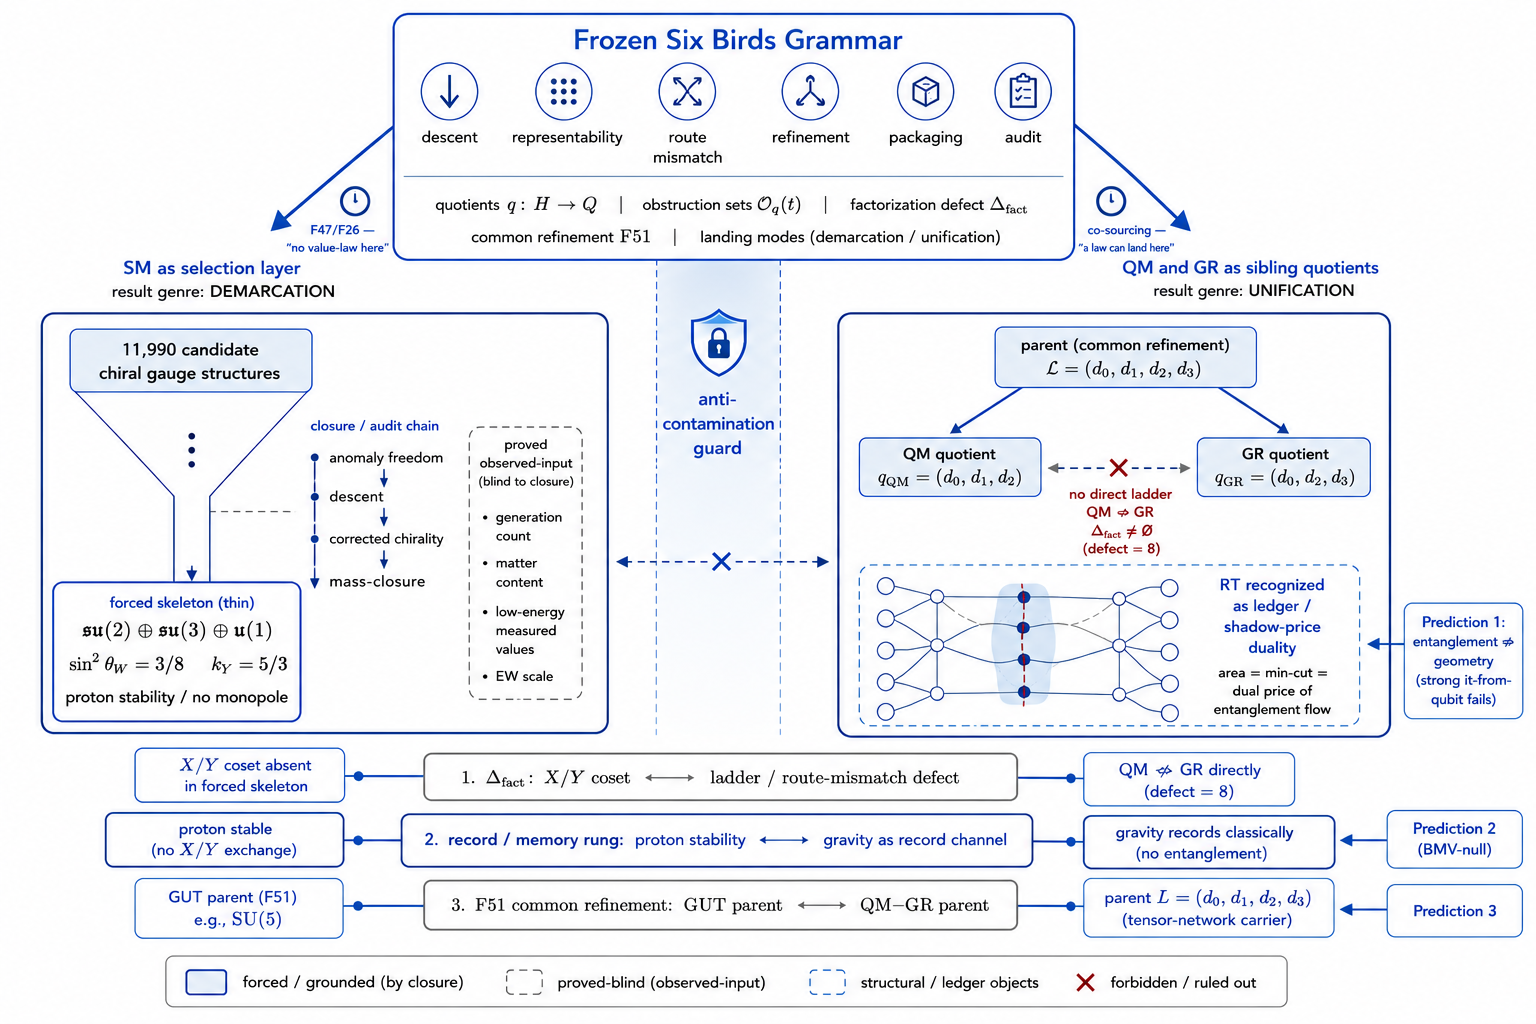
\includegraphics[width=\linewidth]{figures/fig_f1_one_grammar.png}
  \caption{\textbf{The paper's thesis in one panel.} \emph{Center: the grammar (six primitives + F-laws, one box). Two arrows out, through an ``anti-contamination guard'' wall: left to the SM substrate (selection layer) yielding the demarcation stack (§4) and Prediction 3; right to the QM--GR substrate (common refinement) yielding the unification stack (§5) and Predictions 1--2. Beneath each arrow, the prior expectation (F47/F26: ``no value-law here''; co-sourcing: ``a law can land here'') with a timestamp glyph indicating the expectation preceded the result. Connecting the two arms: the cross-track ties of §8.2 drawn as rungs between the substrates --- labeled \(\Delta_{\mathrm{fact}}\), the record rung, F51 --- with the record rung highlighted as the spine of Predictions 2 and 3.}}
  \label{fig:f1}
\end{figure}

\hypertarget{scope-limits-and-falsifiability}{%
\section{Scope, limits, and falsifiability}\label{scope-limits-and-falsifiability}}

This section collects every bound in one place, then gives the claim-by-claim falsifiability table. These are scope
statements, stated flat; none retracts a result.

\hypertarget{the-bounds}{%
\subsection{The bounds}\label{the-bounds}}

\begin{enumerate}
\def\labelenumi{\arabic{enumi}.}
\tightlist
\item
  \textbf{Finite toys; no frame-transfer.} Every computation lives on a declared finite carrier. The carriers \emph{predict}
  and are \emph{falsifiable}, but nothing here is proven about nature. The three predictions of §6 are exactly that ---
  predictions; their status in nature is for experiment and for richer constructions to decide.
\item
  \textbf{Conditional landings are conditional.} Every GROUND/SELECT result rests on a named source: clean-separation on
  record-stability (``why must a universe bear records?'' is the review-judged top of that tower); the QM--GR fork on
  the co-sourcing warrant (which reaches matter-sourced geometry, not the free gravitational sector). The conditions
  are declared, audited, and carried with the results.
\item
  \textbf{Enumeration-strength where stated.} The record-stability implication is \(0/11{,}990\) with bounded outside probes
  --- not yet an all-structures theorem; the open lemma (L60\(\to\)L64: mass-closure charge-linking forbids a second
  neutral record channel in leak-positive substrate closers) is precisely specified and would upgrade Prediction 3
  from enumeration-strength to a structural law. Similar precisely-typed upgrades are open for: exact RT saturation in
  the large-bond limit; the continuum (F43) limit of the discrete Einstein condition; uniqueness of the co-sourcing
  grounding; the all-co-readout form of the monogamy forcing.
\item
  \textbf{\(n=2\) on universality.} Section 8's thesis has exactly two substrates behind it.
\item
  \textbf{Adversarially reviewed, not independently replicated.} Two results settled under adversarial review cycles; no
  independent group has yet re-run the constructions (Appendix B is written to make that easy).
\item
  \textbf{What is \emph{not} claimed anywhere:} a derivation of any measured constant; a solution of quantum gravity; a proof of
  physical proton stability; a universal exact-six reduction; frame-transfer.
\end{enumerate}

\begin{landscape}

\hypertarget{table-t1-every-headline-claim-its-grade-and-what-kills-it}{%
\subsection{Table T1 --- every headline claim, its grade, and what kills it}\label{table-t1-every-headline-claim-its-grade-and-what-kills-it}}

\begin{longtable}[]{@{}llll@{}}
\toprule
\begin{minipage}[b]{0.05\columnwidth}\raggedright
\#\strut
\end{minipage} & \begin{minipage}[b]{0.26\columnwidth}\raggedright
claim\strut
\end{minipage} & \begin{minipage}[b]{0.22\columnwidth}\raggedright
grade\strut
\end{minipage} & \begin{minipage}[b]{0.40\columnwidth}\raggedright
what would falsify / defeat it\strut
\end{minipage}\tabularnewline
\midrule
\endhead
\begin{minipage}[t]{0.05\columnwidth}\raggedright
1\strut
\end{minipage} & \begin{minipage}[t]{0.26\columnwidth}\raggedright
\(\sim99.3\%\) chiral-gauge exclusion → \(\{2|3,\ SU(4)\}\)\strut
\end{minipage} & \begin{minipage}[t]{0.22\columnwidth}\raggedright
COMPUTE (unconditional, in-carrier)\strut
\end{minipage} & \begin{minipage}[t]{0.40\columnwidth}\raggedright
a neutral-closure error: a structure passing all gates outside the family (re-run Appendix B.1)\strut
\end{minipage}\tabularnewline
\begin{minipage}[t]{0.05\columnwidth}\raggedright
2\strut
\end{minipage} & \begin{minipage}[t]{0.26\columnwidth}\raggedright
SM gauge algebra selected on clean-separation\strut
\end{minipage} & \begin{minipage}[t]{0.22\columnwidth}\raggedright
SELECT (conditional)\strut
\end{minipage} & \begin{minipage}[t]{0.40\columnwidth}\raggedright
a clean-separated competitor in-window; or the grounding (row 3) failing\strut
\end{minipage}\tabularnewline
\begin{minipage}[t]{0.05\columnwidth}\raggedright
3\strut
\end{minipage} & \begin{minipage}[t]{0.26\columnwidth}\raggedright
clean-separation grounded in record-stability\strut
\end{minipage} & \begin{minipage}[t]{0.22\columnwidth}\raggedright
GROUND, enumeration-strength\strut
\end{minipage} & \begin{minipage}[t]{0.40\columnwidth}\raggedright
\textbf{one} record-stable structure with \(\Delta_{\mathrm{fact}}\neq\varnothing\) (in-carrier or in any lawful extension); refutation of L60→L64 closes the door the other way\strut
\end{minipage}\tabularnewline
\begin{minipage}[t]{0.05\columnwidth}\raggedright
4\strut
\end{minipage} & \begin{minipage}[t]{0.26\columnwidth}\raggedright
\(\sin^2\theta_W=3/8\), \(k_Y=5/3\) as forced embedding ratios\strut
\end{minipage} & \begin{minipage}[t]{0.22\columnwidth}\raggedright
GROUND (minimal-simple source)\strut
\end{minipage} & \begin{minipage}[t]{0.40\columnwidth}\raggedright
showing the trace ratios depend on an undeclared input; the product control (\(3/23\)) failing to discriminate\strut
\end{minipage}\tabularnewline
\begin{minipage}[t]{0.05\columnwidth}\raggedright
5\strut
\end{minipage} & \begin{minipage}[t]{0.26\columnwidth}\raggedright
\(N_{\mathrm{gen}}\)-blindness, all \(N\)\strut
\end{minipage} & \begin{minipage}[t]{0.22\columnwidth}\raggedright
PROVE-BLIND (theorem)\strut
\end{minipage} & \begin{minipage}[t]{0.40\columnwidth}\raggedright
an \(N\)-sensitive gate in the frozen chain for an even-doublet anomaly-free unit\strut
\end{minipage}\tabularnewline
\begin{minipage}[t]{0.05\columnwidth}\raggedright
6\strut
\end{minipage} & \begin{minipage}[t]{0.26\columnwidth}\raggedright
QM--GR fork (no weak-RT ladder)\strut
\end{minipage} & \begin{minipage}[t]{0.22\columnwidth}\raggedright
COMPUTE (conditional on premise)\strut
\end{minipage} & \begin{minipage}[t]{0.40\columnwidth}\raggedright
a lawful factorization \(q_{\mathrm{GR}}=\phi\circ q_{\mathrm{QM}}\) on the carrier; the nested control failing to flip\strut
\end{minipage}\tabularnewline
\begin{minipage}[t]{0.05\columnwidth}\raggedright
7\strut
\end{minipage} & \begin{minipage}[t]{0.26\columnwidth}\raggedright
common-carrier premise grounded in co-sourcing\strut
\end{minipage} & \begin{minipage}[t]{0.22\columnwidth}\raggedright
GROUND (review-settled)\strut
\end{minipage} & \begin{minipage}[t]{0.40\columnwidth}\raggedright
the warrant shown circular (co-sourcing presupposing the carrier); a complementary pair admitting a joint quotient\strut
\end{minipage}\tabularnewline
\begin{minipage}[t]{0.05\columnwidth}\raggedright
8\strut
\end{minipage} & \begin{minipage}[t]{0.26\columnwidth}\raggedright
RT = ledger/shadow-price duality\strut
\end{minipage} & \begin{minipage}[t]{0.22\columnwidth}\raggedright
RECOGNITION (review-settled)\strut
\end{minipage} & \begin{minipage}[t]{0.40\columnwidth}\raggedright
exact (machine-\(\epsilon\)) saturation at finite \(D\) --- the tautology signature; or geometric side tracking the state spectrum under reseeding\strut
\end{minipage}\tabularnewline
\begin{minipage}[t]{0.05\columnwidth}\raggedright
9\strut
\end{minipage} & \begin{minipage}[t]{0.26\columnwidth}\raggedright
\textbf{Prediction 1: entanglement \(\nRightarrow\) geometry}\strut
\end{minipage} & \begin{minipage}[t]{0.22\columnwidth}\raggedright
FORBIDDEN-RULE (toy)\strut
\end{minipage} & \begin{minipage}[t]{0.40\columnwidth}\raggedright
a non-trivial holographic geometry with injective fingerprint map (zero kernel, no two-sided invisible deformation)\strut
\end{minipage}\tabularnewline
\begin{minipage}[t]{0.05\columnwidth}\raggedright
10\strut
\end{minipage} & \begin{minipage}[t]{0.26\columnwidth}\raggedright
\textbf{Prediction 2: gravity does not entangle (BMV-null)}\strut
\end{minipage} & \begin{minipage}[t]{0.22\columnwidth}\raggedright
FORBIDDEN-RULE (toy; analytically verified)\strut
\end{minipage} & \begin{minipage}[t]{0.40\columnwidth}\raggedright
a confirmed BMV-type detection of gravitationally-induced entanglement; or the coherent-mediator control failing to entangle\strut
\end{minipage}\tabularnewline
\begin{minipage}[t]{0.05\columnwidth}\raggedright
11\strut
\end{minipage} & \begin{minipage}[t]{0.26\columnwidth}\raggedright
\textbf{Prediction 3: records forbid proton decay \& monopoles}\strut
\end{minipage} & \begin{minipage}[t]{0.22\columnwidth}\raggedright
FORBIDDEN-RULE / DEMARCATION (enumeration-strength)\strut
\end{minipage} & \begin{minipage}[t]{0.40\columnwidth}\raggedright
an observed proton decay or magnetic monopole; or one record-stable breaking structure\strut
\end{minipage}\tabularnewline
\begin{minipage}[t]{0.05\columnwidth}\raggedright
12\strut
\end{minipage} & \begin{minipage}[t]{0.26\columnwidth}\raggedright
Bell: carrier \(\neq\) local hidden variable\strut
\end{minipage} & \begin{minipage}[t]{0.22\columnwidth}\raggedright
FORBIDDEN-RULE (recovered Bell + reconciliation)\strut
\end{minipage} & \begin{minipage}[t]{0.40\columnwidth}\raggedright
an admissible joint quotient for complementary accesses; an LHV table reproducing the quantum CHSH\strut
\end{minipage}\tabularnewline
\begin{minipage}[t]{0.05\columnwidth}\raggedright
13\strut
\end{minipage} & \begin{minipage}[t]{0.26\columnwidth}\raggedright
BH information: loss is readout-relative\strut
\end{minipage} & \begin{minipage}[t]{0.22\columnwidth}\raggedright
FORBIDDEN-RULE (static toy)\strut
\end{minipage} & \begin{minipage}[t]{0.40\columnwidth}\raggedright
a gauge-invariant interior observable unrecoverable from the full boundary on the full-rank stratum\strut
\end{minipage}\tabularnewline
\begin{minipage}[t]{0.05\columnwidth}\raggedright
14\strut
\end{minipage} & \begin{minipage}[t]{0.26\columnwidth}\raggedright
\(\Lambda\): no in-layer value-law\strut
\end{minipage} & \begin{minipage}[t]{0.22\columnwidth}\raggedright
DEMARCATION (F50 bounded-moduli)\strut
\end{minipage} & \begin{minipage}[t]{0.40\columnwidth}\raggedright
the frozen closure chain selecting a singleton background\strut
\end{minipage}\tabularnewline
\begin{minipage}[t]{0.05\columnwidth}\raggedright
15\strut
\end{minipage} & \begin{minipage}[t]{0.26\columnwidth}\raggedright
one-grammar thesis\strut
\end{minipage} & \begin{minipage}[t]{0.22\columnwidth}\raggedright
meta-claim, \(n=2\)\strut
\end{minipage} & \begin{minipage}[t]{0.40\columnwidth}\raggedright
a third substrate where the grammar's own genre-expectation fails; or evidence of cross-track contamination\strut
\end{minipage}\tabularnewline
\begin{minipage}[t]{0.05\columnwidth}\raggedright
16\strut
\end{minipage} & \begin{minipage}[t]{0.26\columnwidth}\raggedright
measurement: \(D\)-vs-\(\Sigma_f\) discriminator\strut
\end{minipage} & \begin{minipage}[t]{0.22\columnwidth}\raggedright
structural prediction\strut
\end{minipage} & \begin{minipage}[t]{0.40\columnwidth}\raggedright
a community-accepted single-outcome theory touching neither \(D\) nor \(\Sigma_f\)\strut
\end{minipage}\tabularnewline
\bottomrule
\end{longtable}
\end{landscape}

\hypertarget{why-the-honesty-is-load-bearing}{%
\subsection{Why the honesty is load-bearing}\label{why-the-honesty-is-load-bearing}}

A framework this general invites the Pauli verdict (``not even wrong''). The table above is the rebuttal format: each
claim is either graded as conditional/toy (and says what discharges the condition), or names an observation that would
falsify it. Rows 9, 10, and 11 are the paper's exposure to experiment --- with row 10 (BMV) the nearest-term; rows 3, 6, 7, 8 are
its exposure to construction; row 15 is its exposure to its own program.

\hypertarget{discussion-and-outlook}{%
\section{Discussion and outlook}\label{discussion-and-outlook}}

\hypertarget{what-the-corrections-change}{%
\subsection{What the corrections change}\label{what-the-corrections-change}}

The strongest lesson of the verification campaign is methodological. A finite computation can be exact and still answer
the wrong typed question: aliases can corrupt a denominator; a branch witness can be mistaken for a structure property;
a distance can be called a commutator; a null direction can be quotient gauge; or a solver budget can masquerade as an
existence boundary. Version 2 retains results only after those distinctions are made explicit.

The positive inventory remains useful. The repaired gauge carrier yields a branch-level selection under declared caps;
the regular \(SU(5)\) frame and its coset are explicit exact objects; the content quotient produces one selected orbit;
the \(N\)-copy probe computes real generic ranks; the Boolean access lattice supplies an exact incomparability theorem;
and the min-cut carrier supplies an exact LP dual certificate plus independent contracted-state evidence. None alone is
a theory of nature, but each is a reproducible construction with a clear failure condition.

\hypertarget{nearest-upgrades-precisely-typed-open-problems}{%
\subsection{Nearest upgrades}\label{nearest-upgrades-precisely-typed-open-problems}}

Three upgrades now dominate. First, the 13 residual P1 carriers need either a further exact reduction beyond the five named classes
or a completeness theorem for an exact quotient class; independently, a contracted-state underdetermination
example must be built if the question is to move beyond cuts. Second, BMV relevance requires a dynamical model deriving
record formation, rather than stipulating a measure-and-record channel. Third, the record-stability program requires the
physical invariant algebra and dynamics: UV-to-residual restriction ranks, Grassmann/EOM/syzygy relations, and a
persistence criterion for candidate records.

Other bounded upgrades remain worthwhile: repair the step43 final-carrier counts; replace F-008 summary-reading
validators; establish or refute large-bond RT saturation with a rate; widen the representation and scalar windows; and
generate a physically motivated class of measurement models rather than a two-exemplar taxonomy. A third substrate
could test whether the vocabulary remains useful, but would not by itself prove universality.

\hypertarget{what-kind-of-theory-is-this}{%
\subsection{What kind of framework is this?}\label{what-kind-of-theory-is-this}}

The calculus is not dynamical: it has no Lagrangian, cross-sections, or continuum limit. Its present evidential role is a
finite structural language for asking whether one readout factors through another, whether a candidate set closes, and
which assumptions a recognition imports. The campaign shows both the value and the limit of that language. It can make
hidden quotients and quantifiers visible; it cannot turn an unbuilt physical bridge into a prediction.

\hypertarget{an-invitation}{%
\subsection{An invitation}\label{an-invitation}}

The most useful independent attacks are now concrete: regenerate the repaired carrier under a different declared
quotient; search the 13 P1 residuals for a sixth exact reduction; construct state-level equal-entanglement examples after
physical quotienting; derive a gravitational record channel from dynamics; or compute the restriction and relation
structure of the record invariant ring. A disagreement with any exported finite table is a direct reproducibility
failure. A physical result addresses the open program only when the missing carrier-to-physics map is supplied.

\hypertarget{conclusion}{%
\section{Conclusion}\label{conclusion}}

On declared finite carriers, this paper provides a conjugation-consistent branch-typed
gauge selection, a witness-independent single-factor toy theorem, an explicitly constructed \(SU(5)\) frame and coset,
a unique content orbit under a named quotient, generic mass ranks for materialized \(N=1,\ldots,4\), an exact abstract
partition-incomparability theorem with conditional field provenance, and a finite-graph min-cut/LP-duality
recognition supported by contracted-state and monogamy controls. Every statement carries its caps, quotient conventions,
imports, sample bounds, or depth limit.

The exact negative findings are results in their own right, and they bound what the framework can presently claim: the
quantize/curve conditional-mean completions commute, so no route-mismatch explanation of quantum gravity's difficulty is
available at this level; the bounded record-stability census is token-definition-sensitive; Born and area do not share
the tested composition law; the linearized-Einstein response does not match at an honest nondegenerate base point; and
the generation grammar neither stays blind to \(N\) nor selects \(N=3\).

The graph result gives nineteen exact same-graph fibers whose corresponding endpoint forward-reachability sets
are disjoint under four directed reductions and bidirectional Delta-Y/Y-Delta, with symmetric-closure orbit disjointness
open. The state result gives six exact noninjective fibers of the joint complete-cut/state map and the general
\(C2\_L1\) gauge-collapse lemma: the six pairs are not inequivalent tensor-network presentations. No physically complete
bulk gauge relation or bulk-geometry underdetermination theorem is established.

P1's two finite subproblems are completed at that strength, while symmetric closure and the broader physical
and bulk interpretation remain open. P2 and P3 remain construction programs: dynamical gravitational record formation and
dynamical persistence in the scalar-dressed record algebra. The common grammar has not forced their answers. Its
demonstrated contribution is narrower: it organized two finite construction programs and, under sustained adversarial
scrutiny, exposed exactly where stronger claims would fail.


\appendix
\hypertarget{the-calculus-formally-working-subset}{%
\section{the calculus, formally (working subset)}\label{the-calculus-formally-working-subset}}

This appendix states, at usable precision, every formal object the body relies on. Full development: Foundations II--IV~\citep{Tsiokos_FoundationsII,Tsiokos_FoundationsIII,Tsiokos_FoundationsIV}.

\hypertarget{descent-and-obstruction}{%
\subsection{Descent and obstruction}\label{descent-and-obstruction}}

For a surjection \(q:H\to Q\) and readout \(t:H\to T\):

\[
t \text{ descends} \iff \mathcal O_q(t) = \{(h,h'): q(h)=q(h') \wedge t(h)\neq t(h')\} = \varnothing
\iff \exists\,\bar t:Q\to T,\ \bar t\circ q = t .
\]

Both directions are finite checks on \(H\times H\) (choose representatives; well-definedness is exactly
fiber-constancy).

\hypertarget{strict-extension-and-the-factorization-defect-fiii-thms-1213}{%
\subsection{Strict extension and the factorization defect (FIII Thms 12--13)}\label{strict-extension-and-the-factorization-defect-fiii-thms-1213}}

For maps \(\pi_0:S\to O_0\), \(\pi_1:S\to O_1\) on a finite carrier:

\[
\Delta_{\mathrm{fact}}(\pi_0,\pi_1) = \{(s,s'): \pi_0(s)=\pi_0(s') \wedge \pi_1(s)\neq\pi_1(s')\},
\qquad
\Delta_{\mathrm{fact}}\neq\varnothing \iff \nexists\,\phi:\ \pi_1 = \phi\circ\pi_0 .
\]

Used as: the \(X/Y\) coset (§4: witnesses of the clean-separation defect); GUT\(\leftrightarrow\)SM non-relabeling
(\(\Delta_{\mathrm{fact}}(\mathrm{SM},\mathrm{GUT})=15\), reverse \(=0\)); the QM--GR ladder defect (\(8\) witnesses).

\hypertarget{non-commuting-completions-fiii-thms-910}{%
\subsection{Non-commuting completions (FIII Thms 9--10)}\label{non-commuting-completions-fiii-thms-910}}

There exist idempotents \(E_1,E_2\) on a finite carrier with \(E_1E_2\neq E_2E_1\); the route-mismatch defect
\(\Delta_3^{\mathrm{comp}}(E_1,E_2)=\{c: E_1E_2(c)\neq E_2E_1(c)\}\) is non-empty iff they fail to commute. Minimal
witness: \(C=\mathcal P(\{a,b,c\})\), \(E_1(S)=S\cup\{b\}\) if \(a\in S\) else \(S\); \(E_2(S)=S\cup\{c\}\) if \(b\in S\) else \(S\);
then \(E_1E_2(\{a\})=\{a,b\}\neq\{a,b,c\}=E_2E_1(\{a\})\). Reading: route mismatch is a real typed defect even when each
completion is individually exact --- the calculus's typing of non-renormalizability (§5.1).

\hypertarget{the-six-primitives-and-the-no-algebra-theorem}{%
\subsection{The six primitives and the no-algebra theorem}\label{the-six-primitives-and-the-no-algebra-theorem}}

\(\mathbb P=\{P_1,\dots,P_6\}\) (descent, representability, route mismatch, refinement, packaging, audit) are role
labels for typed judgments. Theorem-grade exclusions (FIII): no total binary operation \(*:\mathbb P^2\to\mathbb P\)
decodes judgment status (no total six-symbol algebra); no universal claim that all structure decomposes into the six.
Directed-cell notation \(P_i \leftarrow P_j\) names a typed, individually-audited judgment, never a product.

\hypertarget{the-f-laws-used-in-this-paper-one-line-formal-cores}{%
\subsection{The F-laws used in this paper (one-line formal cores)}\label{the-f-laws-used-in-this-paper-one-line-formal-cores}}

\begin{longtable}[]{@{}lll@{}}
\toprule
\begin{minipage}[b]{0.23\columnwidth}\raggedright
law\strut
\end{minipage} & \begin{minipage}[b]{0.51\columnwidth}\raggedright
statement (core)\strut
\end{minipage} & \begin{minipage}[b]{0.19\columnwidth}\raggedright
used in\strut
\end{minipage}\tabularnewline
\midrule
\endhead
\begin{minipage}[t]{0.23\columnwidth}\raggedright
\textbf{F23} probability\strut
\end{minipage} & \begin{minipage}[t]{0.51\columnwidth}\raggedright
a readout unresolved on the fiber of \(q\) admits a \emph{stable} weight \(\Pr_{q,r}(a,v)=m(\lambda(a))(\{h: q(h)=a, r(h)=v\})\)\strut
\end{minipage} & \begin{minipage}[t]{0.19\columnwidth}\raggedright
§5.4 (Born ledger)\strut
\end{minipage}\tabularnewline
\begin{minipage}[t]{0.23\columnwidth}\raggedright
\textbf{F26/F47} contingency \& fine-tuning\strut
\end{minipage} & \begin{minipage}[t]{0.51\columnwidth}\raggedright
no value-law lands on a contingent (moduli) selection; fine-tuning = small selector region\strut
\end{minipage} & \begin{minipage}[t]{0.19\columnwidth}\raggedright
§4.6, §7.3, §8.4\strut
\end{minipage}\tabularnewline
\begin{minipage}[t]{0.23\columnwidth}\raggedright
\textbf{F27} conservation\strut
\end{minipage} & \begin{minipage}[t]{0.51\columnwidth}\raggedright
a charge is conserved iff it descends through the orbit quotient (obstruction \(=0\))\strut
\end{minipage} & \begin{minipage}[t]{0.19\columnwidth}\raggedright
§4.4, §6.3 (baryon number)\strut
\end{minipage}\tabularnewline
\begin{minipage}[t]{0.23\columnwidth}\raggedright
\textbf{F34} information loss\strut
\end{minipage} & \begin{minipage}[t]{0.51\columnwidth}\raggedright
\(\mathrm{Recoverable}(\sigma,\tau,\rho) \iff \mathcal O_\rho=\{(h,h'):\rho(\tau h)=\rho(\tau h') \wedge \sigma(h)\neq\sigma(h')\}=\varnothing\); loss legitimate iff later identifications are invisible to \(\sigma\)\strut
\end{minipage} & \begin{minipage}[t]{0.19\columnwidth}\raggedright
§7.2\strut
\end{minipage}\tabularnewline
\begin{minipage}[t]{0.23\columnwidth}\raggedright
\textbf{F37} complementarity\strut
\end{minipage} & \begin{minipage}[t]{0.51\columnwidth}\raggedright
\(q_A \perp q_B \iff \nexists (J,j,a,b):\ a\circ j=q_A \wedge b\circ j=q_B\) (no admissible joint quotient)\strut
\end{minipage} & \begin{minipage}[t]{0.19\columnwidth}\raggedright
§5.3, §7.1\strut
\end{minipage}\tabularnewline
\begin{minipage}[t]{0.23\columnwidth}\raggedright
\textbf{F39} entropy\strut
\end{minipage} & \begin{minipage}[t]{0.51\columnwidth}\raggedright
\(E(q)\) = fiber volume; chain rule \(E(q_C)=E(q_F)\odot m\); monotone under coarsening\strut
\end{minipage} & \begin{minipage}[t]{0.19\columnwidth}\raggedright
§5.4 (area ledger)\strut
\end{minipage}\tabularnewline
\begin{minipage}[t]{0.23\columnwidth}\raggedright
\textbf{F48} gluing/topology\strut
\end{minipage} & \begin{minipage}[t]{0.51\columnwidth}\raggedright
global obstruction as non-trivial gluing class (monopole obstruction \(=0\) in the clean branch)\strut
\end{minipage} & \begin{minipage}[t]{0.19\columnwidth}\raggedright
§4.4, §6.3\strut
\end{minipage}\tabularnewline
\begin{minipage}[t]{0.23\columnwidth}\raggedright
\textbf{F49} common source\strut
\end{minipage} & \begin{minipage}[t]{0.51\columnwidth}\raggedright
\(\mathrm{LocallyExplainable}(\kappa) \iff \mathrm{CommonSource}(\sigma) \vee \mathrm{InterfaceFactorization}(\iota)\); else statused nonlocal residual\strut
\end{minipage} & \begin{minipage}[t]{0.19\columnwidth}\raggedright
§7.1\strut
\end{minipage}\tabularnewline
\begin{minipage}[t]{0.23\columnwidth}\raggedright
\textbf{F50} background selection\strut
\end{minipage} & \begin{minipage}[t]{0.51\columnwidth}\raggedright
descended background \(b\): \textbf{necessary} (\(b\) constant) xor \textbf{moduli} (\(\exists m,m': b(m)\neq b(m')\)); \textbf{vacuum} iff \(V=\{m_*\}\)\strut
\end{minipage} & \begin{minipage}[t]{0.19\columnwidth}\raggedright
§7.3\strut
\end{minipage}\tabularnewline
\begin{minipage}[t]{0.23\columnwidth}\raggedright
\textbf{F51} unification\strut
\end{minipage} & \begin{minipage}[t]{0.51\columnwidth}\raggedright
parent \(Q_U\) with commuting squares \(\pi_A\circ q_U = q_A\circ\iota_A\), \(\pi_B\circ q_U = q_B\circ\iota_B\) + status-compatible claim lifts\strut
\end{minipage} & \begin{minipage}[t]{0.19\columnwidth}\raggedright
§4.4, §5.2, §5.4\strut
\end{minipage}\tabularnewline
\bottomrule
\end{longtable}

\hypertarget{landing-modes-and-audit-gates-operational-definitions}{%
\subsection{Landing modes and audit gates (operational definitions)}\label{landing-modes-and-audit-gates-operational-definitions}}

\textbf{Modes.} COMPUTE (value/verdict from the construction); SELECT (choice on declared conditions); PROVE-BLIND
(invariance theorem ⇒ observed-input); GROUND (condition supplied as down-shadow of a named higher source; carries
source-warrant + theorem-strength caveats); RECOGNITION (known result reproduced as a law-instance, non-circularly);
FORBIDDEN-RULE/DEMARCATION (computed exclusion/classification with can-fail control).

\textbf{Gates} (all mechanical; validators enforce): \emph{anti-tautology} --- target not definitionally equal to its evidence;
\emph{anti-circularity} --- each hypothesis independently satisfiable by a conclusion-violating structure (exhibited);
\emph{frozen-machinery} --- imports SHA-256-pinned, no retuning; \emph{can-fail control} --- a configuration on which the claim fails;
\emph{no-overclaim} --- artifact text checked against a blocklist; \emph{anti-contamination} (cross-track) --- substrate-foreign
tokens fail the build.

\hypertarget{the-key-derived-quantities-of-the-body}{%
\subsection{The key derived quantities of the body}\label{the-key-derived-quantities-of-the-body}}

\begin{itemize}
\tightlist
\item
  \textbf{Embedding ratios} (§4.4): over one SM generation,
  \(\operatorname{Tr}T_3^2 = 3\!\cdot\!2\!\cdot\!\tfrac14 + 2\!\cdot\!\tfrac14\!\cdot\!2 = 2\) (quark + lepton doublets),
  \(\operatorname{Tr}Q^2 = \tfrac83 + \tfrac23 + 2 = \tfrac{16}{3}\), hence \(\sin^2\theta_W = 3/8\); hypercharge
  normalization \(k_Y = 5/3\) from \(\operatorname{Tr}Y^2 = 5/6\). Control: a non-simple product parent yields \(3/23\).
\item
  \textbf{RT/shadow price} (§5.4): for entanglement flow with capacities \(b\), strong duality gives
  \(\max(\text{flow}) = \min(\text{cut})\) and the cut value is the dual optimum --- the shadow price
  \(\lambda = \partial \Phi^*/\partial b\) of the capacity constraints; ``area'' is that price.
\item
  \textbf{Monogamy} (§5.4, §6.1): \(I_3 \le 0\) for min-cut-realizable entropy vectors; GHZ\(_4\) has \(I_3 = +\log 2\).
\item
  \textbf{CHSH} (§7.1): local bound \(\max_{\lambda\in\{\pm1\}^4} |E_{00}+E_{01}+E_{10}-E_{11}| = 2\) (16-strategy
  enumeration); Bell state with \(a_0=Z, a_1=X, b_{0,1}=(Z\pm X)/\sqrt2\) gives \(2\sqrt2\).
\item
  \textbf{Prediction kernels} (§6): \(J = \partial\mathcal E/\partial w\) (central differences, non-degenerate base);
  \(\dim\ker J = 5\); clean-shadow edges = \(\{e: \mathcal E(w \pm \delta\,\hat e) = \mathcal E(w)\ \text{exactly},\
  \delta \in [0.05, 0.15]\}\), count \(2\) per seed.
\end{itemize}

\section{Constructions and reproducibility}\label{toy-constructions-reproducibility}

The historical construction tracks live under \nolinkurl{physics_atlas/}; the controlling repairs and probes live under
\nolinkurl{review_2026/}; the construction programs live under \nolinkurl{open_programs/}. Where a historical headline
and a controlling repair disagree, the repair and the claims registry \nolinkurl{review_2026/CLAIMS_REGISTRY.md}
control. Validators vary in strength: many historical scripts check deterministic artifacts, while the strongest
rebuild their entire result in memory and compare every output byte for byte.

\subsection{Entry points for the controlling results}

\begin{center}
\small
\begin{longtable}[]{@{}p{0.29\linewidth}p{0.42\linewidth}p{0.21\linewidth}@{}}
\toprule
result & artifact directory & validator (\texttt{--self})\\
\midrule
\endhead
gauge carrier, branch census, scalar pairs &
\nolinkurl{review_2026/repairs/s1_carrier_reconstruction/} &
\nolinkurl{run_s1_carrier_reconstruction_v3.py}\\
\(SU(5)\) generators, ratios, coset, F27/F48 &
\nolinkurl{review_2026/repairs/s3_generator_construction/} &
\nolinkurl{run_s3_generator_construction_v2.py}\\
content quotient, mass rank, \(N\)-copy probe &
\nolinkurl{review_2026/repairs/s4_content_quotient/} &
\nolinkurl{run_s4.py}\\
F24/F47 architecture and surface &
\nolinkurl{review_2026/repairs/s5_f24_f47/} &
\nolinkurl{run_s5.py}\\
record-token census and ablations &
\nolinkurl{review_2026/repairs/s6_record_grammar_ablation/} &
\nolinkurl{run_s6_record_grammar_ablation_v3.py}\\
field provenance and partition lattice &
\nolinkurl{review_2026/repairs/q1_access_provenance/} &
\nolinkurl{run_q1.py}\\
route-mismatch commutation &
\nolinkurl{review_2026/repairs/q2_route_mismatch/} &
\nolinkurl{run_q2.py}\\
min-cut LP duality, response, composition &
\nolinkurl{review_2026/repairs/q5_lp_duality/} &
\nolinkurl{run_q5.py}\\
adaptive F50 convergence and stability &
\nolinkurl{review_2026/repairs/q7_f50_convergence/} &
\nolinkurl{run_q7.py}\\
F34 factorization theorem, rank certificates, partial-readout witness &
\nolinkurl{review_2026/repairs/f34_exact_factorization/} &
\nolinkurl{run_exact_factorization.py}\\
five-class P1 quotient search &
\nolinkurl{review_2026/probes/p1_kernel_quotient/} &
\nolinkurl{run_active_cut_quotient_v3.py}\\
P1 graph level: forward reachability &
\nolinkurl{open_programs/prog3_cut_fingerprints/step2_orbit_saturation/} &
\nolinkurl{run_step2.py}\\
P1 graph level: symmetric-closure obstruction &
\nolinkurl{open_programs/prog3_cut_fingerprints/step3_symmetric_closure/} &
\nolinkurl{run_step3.py}\\
P1 state level: finite \texttt{C2\_L1} classification &
\nolinkurl{open_programs/prog2_state_underdetermination/step5_family_gauge_classification/} &
\nolinkurl{run_step5.py}\\
P1 state level: gauge-collapse lemma &
\nolinkurl{open_programs/prog2_state_underdetermination/step6_exact_gauge_collapse/} &
\nolinkurl{run_step6.py}\\
\bottomrule
\end{longtable}
\end{center}

Each directory contains its design choices, literal dependency pins, schema, result tables, and a findings note; the
caps and conventions stated in the body are also machine-readable there. The F34 directory additionally contains the
written proof of Theorem~\ref{thm:f34} (\nolinkurl{PROOF.txt}). The proof is general linear algebra; the Python code
checks exact finite instances and is not a Lean mechanization of the universal statement.

\subsection{Independent checks}

The mathematics review in \nolinkurl{review_2026/mathematics_audit_20261003/} adds checks that do not reuse
production code: the weight-character representation oracle of Section~\ref{finite-frozen-carriers}, tampering
controls for the strengthened validators, regressions of the gauge-collapse certificate on every connected labelled
simple graph with at most four vertices, and a per-claim coverage file for all \(42\) registry records. They are
reproduced by
\begin{verbatim}
python3 review_2026/mathematics_audit_20261003/run_checks.py \
    --output /tmp/sm-qm-gr-audit.json
\end{verbatim}
Adding \texttt{--all} also sweeps the controlling and historical validators. The runner works in separate scratch
copies built from tracked, non-ignored files, so a missing local artifact cannot silently supply evidence.

\subsection{Historical track rebuilds and an external corpus variable}

Step validators in a clean checkout resolve repository-internal sources relative to their own files. The usual
pattern is
\begin{verbatim}
cd physics_atlas/thread_<track>/steps/<step_dir>
python3 run_stepNN.py --self
\end{verbatim}
Four historical QM--GR build drivers (steps 51--54) also reproduce hashes of Foundations III/IV corpus \texttt{.tex}
files that are not distributed here. Rebuilding those rows requires an explicit external root,
\begin{verbatim}
SIX_BIRDS_PAPERS_ROOT=/path/to/six-birds-papers \
  python3 <step51--54-build-driver>.py
\end{verbatim}
Without it, those drivers stop before writing partial artifacts and name the missing file. The variable is not needed
to validate the released artifacts or to run repairs that only import compute functions; it is a provenance
dependency, not evidence that this checkout contains the external corpus.

\subsection{Validator caveats}

The repository is not uniformly self-verifying, and it is not a tamper-evident freeze.

\begin{itemize}\tightlist
\item \textbf{Summary-reading validators.} The validators of the historical multi-factor window-closure steps
  (steps 43 and 44 of the SM cluster) and some analogues check stored audit tables instead of rebuilding every
  load-bearing computation. The step-43 numerical census counts are also stale relative to the final carrier: a
  current-engine probe supports its \(N\le6\) family conclusion, but a final-carrier rebuild remains to be done. By
  contrast, the step-61 validator (single-factor theorem) rebuilds every released non-code artifact in a temporary directory,
  compares bytes, and constructs the actual witness pairs.
\item \textbf{In-place regeneration.} Some \texttt{--self} validators regenerate artifacts in place, so they are not
  idempotent checks of a release tree. A race in a parallel pool was observed once. Run sweeps in isolated scratch
  copies.
\item \textbf{Pins.} The historical step-69 score source is pinned by a literal reviewed digest, so changing the
  source fails even if the stored conclusion is left unchanged. That step's record implication is superseded by the
  record census of Section~\ref{record-stability-open-program}. The preregistration \texttt{SHA256SUMS} primer entry
  names a file absent from the release, and the freeze gate is a consistency check, not a cryptographic or externally
  timestamped freeze.
\item \textbf{Tracked inputs only.} The QM--GR step-27 and step-28 validators reconstruct their operators and histories
  from tracked inputs (step 28 checks every stored history state and potential), and the evidence log required by the
  P1 state-level step-6 validator is tracked. The compatible-clock constraints of steps 27--28 are finite
  constructions whose compatibility is engineered, not a derived clock dynamics.
\item \textbf{P1 search scope.} The initial P1 probe used a declared three-round \(\Delta\)--Y/Y--\(\Delta\) search. The
  controlling validator rebuilds nineteen exact fibers and exhausts their forward reachability under four directed
  reductions and bidirectional \(\Delta\)--Y/Y--\(\Delta\), up to terminal-label-fixed exact weighted isomorphism.
  Symmetric-closure orbit disjointness, paths through tied-minimizer presentations, and other transformations remain
  open.
\end{itemize}

The Q5 replay policy separates exact discrete artifacts, which are compared byte for byte, from floating-point
summaries, whose numeric fields use tight declared tolerances while all non-numeric structure stays exact
(\nolinkurl{review_2026/repairs/q5_lp_duality/reproducibility_policy.md}). The registry records, for every claim, its
wording, status, evidence type, supersession history, controlling source, and validator.

\subsection{Paper build}

The modular manuscript builds with \texttt{make paper-build}, which compiles \nolinkurl{paper/main.tex} and writes
\nolinkurl{paper/build/main_flat.tex}; the tracked root \texttt{.tex} file is copied from that flattened output. All
figures are drawn in TikZ inside the source, so the flattened file needs no external image files. The Qeios bundle is
regenerated from the same sources.

\hypertarget{adversarial-audit-trail-what-was-rejected-and-why}{%
\section{adversarial audit trail: what was rejected, and why}\label{adversarial-audit-trail-what-was-rejected-and-why}}

We publish the program's rejected constructions deliberately. A framework as expressive as this one can manufacture
results in either direction --- toward novelty or toward the safety of recovery --- and the only durable defense is a
record showing both failure modes being caught. Every entry below was detected by the audit gates of §2.4/§3 (or by
line-by-line review against them) and rejected. Some replacements were themselves overturned by the verification
campaign; this appendix preserves that chronology rather than calling every intermediate replacement certified.

\begin{landscape}

\hypertarget{tautologies-the-target-equal-to-its-evidence}{%
\subsection{Tautologies (the target equal to its evidence)}\label{tautologies-the-target-equal-to-its-evidence}}

\begin{longtable}[]{@{}llll@{}}
\toprule
\begin{minipage}[b]{0.19\columnwidth}\raggedright
rejected construction\strut
\end{minipage} & \begin{minipage}[b]{0.26\columnwidth}\raggedright
the defect\strut
\end{minipage} & \begin{minipage}[b]{0.21\columnwidth}\raggedright
the tell\strut
\end{minipage} & \begin{minipage}[b]{0.26\columnwidth}\raggedright
the accepted replacement\strut
\end{minipage}\tabularnewline
\midrule
\endhead
\begin{minipage}[t]{0.19\columnwidth}\raggedright
area--entropy ``law'' v1 (QM--GR)\strut
\end{minipage} & \begin{minipage}[t]{0.26\columnwidth}\raggedright
\emph{area} defined as boundary cell-count and \(S\) as cells \(\times \ln 2\) --- equality by construction\strut
\end{minipage} & \begin{minipage}[t]{0.21\columnwidth}\raggedright
validator would have passed; caught by reading the build: no can-fail case possible\strut
\end{minipage} & \begin{minipage}[t]{0.26\columnwidth}\raggedright
saturable bound \(S(A)\le\mathrm{mincut}\) with required strict-gap controls (§5.4)\strut
\end{minipage}\tabularnewline
\begin{minipage}[t]{0.19\columnwidth}\raggedright
area--entropy ``law'' v2\strut
\end{minipage} & \begin{minipage}[t]{0.26\columnwidth}\raggedright
bulk dimensions set equal to state dimensions, forcing the match\strut
\end{minipage} & \begin{minipage}[t]{0.21\columnwidth}\raggedright
same\strut
\end{minipage} & \begin{minipage}[t]{0.26\columnwidth}\raggedright
same\strut
\end{minipage}\tabularnewline
\begin{minipage}[t]{0.19\columnwidth}\raggedright
Born--area ``one ledger'' v1\strut
\end{minipage} & \begin{minipage}[t]{0.26\columnwidth}\raggedright
\(S_{F39}\) computed from the Schmidt spectrum, \(H_{F23}\) from eigenvalues of \(\rho_A\) --- \emph{the same spectrum twice} (von Neumann \(=\) Shannon of squared singular values)\strut
\end{minipage} & \begin{minipage}[t]{0.21\columnwidth}\raggedright
machine-\(\epsilon\) ``coincidence'' (\(8.9\times10^{-16}\)) --- an identity, true for any pure state, zero co-sourcing content\strut
\end{minipage} & \begin{minipage}[t]{0.26\columnwidth}\raggedright
geometric min-cut as the \(F39\) side: seed-invariant (\(\log 3\)) while \(S_{\mathrm{Born}}\) varies; strict saturation gaps; validator now \textbf{fails on} machine-equality (§5.4)\strut
\end{minipage}\tabularnewline
\begin{minipage}[t]{0.19\columnwidth}\raggedright
first-law ``consequence'' (δS relabeling)\strut
\end{minipage} & \begin{minipage}[t]{0.26\columnwidth}\raggedright
\(\delta S = \delta\langle H_{\mathrm{mod}}\rangle\) restated on a density matrix disconnected from the carrier --- no new checkable content\strut
\end{minipage} & \begin{minipage}[t]{0.21\columnwidth}\raggedright
correct but empty: nothing could have failed\strut
\end{minipage} & \begin{minipage}[t]{0.26\columnwidth}\raggedright
the entropy-cone/MMI consequence with the GHZ violator (§5.4)\strut
\end{minipage}\tabularnewline
\bottomrule
\end{longtable}

\hypertarget{circularity-and-hardcoding-the-load-bearing-clause-doing-no-work}{%
\subsection{Circularity and hardcoding (the load-bearing clause doing no work)}\label{circularity-and-hardcoding-the-load-bearing-clause-doing-no-work}}

\begin{longtable}[]{@{}llll@{}}
\toprule
\begin{minipage}[b]{0.19\columnwidth}\raggedright
rejected construction\strut
\end{minipage} & \begin{minipage}[b]{0.26\columnwidth}\raggedright
the defect\strut
\end{minipage} & \begin{minipage}[b]{0.21\columnwidth}\raggedright
the tell\strut
\end{minipage} & \begin{minipage}[b]{0.26\columnwidth}\raggedright
the accepted replacement\strut
\end{minipage}\tabularnewline
\midrule
\endhead
\begin{minipage}[t]{0.19\columnwidth}\raggedright
monogamy forcing v1 (F51)\strut
\end{minipage} & \begin{minipage}[t]{0.26\columnwidth}\raggedright
``forced\(\,=\,\)compatible \(\wedge\, I_3\le0\)'' with the compatibility flag \textbf{constantly true}; broken-compatibility control written as \textbf{literal} booleans\strut
\end{minipage} & \begin{minipage}[t]{0.21\columnwidth}\raggedright
the forcing reduced to the known fact ``holographic states obey MMI''; the control never computed\strut
\end{minipage} & \begin{minipage}[t]{0.26\columnwidth}\raggedright
historical computed compatibility control; the later composition probe still refutes a universal shared Born--area law (§5.4)\strut
\end{minipage}\tabularnewline
\begin{minipage}[t]{0.19\columnwidth}\raggedright
clean-separation ``grounding'' v1 (SM)\strut
\end{minipage} & \begin{minipage}[t]{0.26\columnwidth}\raggedright
the internal grounding assumed clean separation\strut
\end{minipage} & \begin{minipage}[t]{0.21\columnwidth}\raggedright
anti-circularity gate: a hypothesis not independently satisfiable by a violating structure\strut
\end{minipage} & \begin{minipage}[t]{0.26\columnwidth}\raggedright
historical record-stability repair; later scalar-dressed token census refutes the forcing (§4.5)\strut
\end{minipage}\tabularnewline
\begin{minipage}[t]{0.19\columnwidth}\raggedright
SM ``candidate-law generation'' (early)\strut
\end{minipage} & \begin{minipage}[t]{0.26\columnwidth}\raggedright
a \texttt{total\_slots\ =\ 5} prior and an exterior/GUT-shaped predicate smuggled the answer\strut
\end{minipage} & \begin{minipage}[t]{0.21\columnwidth}\raggedright
caught by adversarial review + internal re-audit; demoted\strut
\end{minipage} & \begin{minipage}[t]{0.26\columnwidth}\raggedright
the certified conjugation-consistent carrier and branch-complete selection (§4.2--4.3)\strut
\end{minipage}\tabularnewline
\begin{minipage}[t]{0.19\columnwidth}\raggedright
assorted (SM)\strut
\end{minipage} & \begin{minipage}[t]{0.26\columnwidth}\raggedright
a shape-flavored \nolinkurl{factor_local_breaking} predicate; a minimality ``currency'' rescue; an \(SU(2)\)-cubic-anomaly bug\strut
\end{minipage} & \begin{minipage}[t]{0.21\columnwidth}\raggedright
each detected in review; each would have faked a landing\strut
\end{minipage} & \begin{minipage}[t]{0.26\columnwidth}\raggedright
reconstructed carrier; the published \(11{,}990\) denominator and exclusions do not survive (§4.2)\strut
\end{minipage}\tabularnewline
\bottomrule
\end{longtable}
\end{landscape}

\hypertarget{rigging-toward-a-desired-verdict-both-directions-prediction-1s-four-attempts}{%
\subsection{Rigging toward a desired verdict --- both directions (the P1 sequence)}\label{rigging-toward-a-desired-verdict-both-directions-prediction-1s-four-attempts}}

The entanglement-kernel claim (§6.1) passed through four historical constructions; the fourth was accepted before exact
quotient review and is now superseded.

\begin{enumerate}
\def\labelenumi{\arabic{enumi}.}
\tightlist
\item
  \textbf{Rigged toward the positive.} A bespoke hand-built graph (edge roles literally named \texttt{active\_bottleneck},
  \texttt{hidden\_half}) with three parallel channels --- the ``invisible mode'' engineered into the carrier; and the ``bulk
  invariant'' that moved was a single edge's weight relabeled as a distance. \emph{Defect class: manufactured witness.}
\item
  \textbf{Rigged toward the deflationary.} On the honest carrier, the genuine-mode dimension was \textbf{hardcoded to zero}
  (a dead conditional over an empty basis), and the scoring filter (``only multi-edge geodesics count; volume is
  slack'') was chosen so the computed kernel could not count. \emph{Defect class: verdict-by-filter; hardcoded score.}
\item
  \textbf{Inflated by a degeneracy artifact.} At the uniform-weight base point (all 14 edges equal, all cuts tied), a
  one-sided forward-difference Jacobian reported nullity 6 --- but every ``kernel'' direction changed the fingerprint at
  first order (residuals scaling linearly with step: \(2.3\times10^{-1}, 2.3\times10^{-3}, 2.3\times10^{-5}\) at
  \(\epsilon = 10^{-1,-3,-5}\)), and single edges were invisible in one direction only (cut slack). \emph{Defect class:
  linearization artifact at a non-generic point.}
\item
  \textbf{Historically accepted, then overturned.} Generic tie-broken geometries; two-sided central differences;
  both-direction finite-range invisibility and a tree control produced nullity \(5/5/5\). Exact series/parallel quotienting
  later showed all five directions were parameterization gauge. The maintained five-class search leaves 13 explicitly
  unclassified residual carriers, not a physical prediction.
\end{enumerate}

\hypertarget{what-the-trail-shows}{%
\subsection{What the trail shows}\label{what-the-trail-shows}}

Three observations. (i) The gates caught failures in both directions, but not always immediately. (ii)
Validator-pass is necessary, never sufficient: semantic defects survived green historical validators. (iii) The paper
therefore claims no ``three surviving predictions.'' It reports certified finite constructions and open programs, with the
specific failed definitions and controls retained as regressions.

\section{Notation and key numbers}\label{notation-the-six-primitives-at-a-glance}

\subsection{Recurring symbols}\label{recurring-symbols}

\begin{center}
\small
\begin{longtable}[]{@{}p{0.27\linewidth}p{0.55\linewidth}p{0.1\linewidth}@{}}
\toprule
symbol & meaning & first use\\
\midrule
\endhead
\(H,\ q,\ Q,\ t\) & carrier, access map, layer, readout & \S\ref{layers-quotients-and-descent}\\
\(\mathcal O_q(t)\) & obstruction set: witnesses that \(t\) does not descend through \(q\) & \S\ref{layers-quotients-and-descent}\\
\(\Deltafact(\pi_0,\pi_1)\) & factorization defect: witnesses that \(\pi_1\) is not a function of \(\pi_0\) & \S\ref{layers-quotients-and-descent}\\
\(P_1,\dots,P_6\) & the six role names (descent, representability, route mismatch, refinement, packaging, audit) & \S\ref{the-six-primitive-roles}\\
F\(n\) & structural law \(n\) of the catalog (Appendix~\ref{the-f-laws-used-in-this-paper-one-line-formal-cores}) & \S\ref{the-six-primitive-roles}\\
\(2|3\) & gauge structures whose nonabelian factors are \(SU(2)\) and \(SU(3)\) & \S\ref{conditional-selection-of-mathfraksu2oplusmathfraksu3oplusmathfraku1}\\
\(\Delta_3^{\mathrm{comp}}(E_1,E_2)\) & route-mismatch defect of two idempotent completions & \S\ref{locating-the-obstruction-the-route-mismatch}\\
\(L=(d_0,d_1,d_2,d_3)\) & the QM--GR common refinement; \(q_{\rm QM}=(d_0,d_1,d_2)\), \(q_{\rm GR}=(d_0,d_2,d_3)\) & \S\ref{the-resolution-a-fork-not-a-ladder}\\
\(\psi,\ V_0\) & field and background potential of the \(54\)-record construction & \S\ref{the-resolution-a-fork-not-a-ladder}\\
\(T_{\mathrm{QG\text{-}NoGo}}\) & narrow statement about two fused or stapled routes & \S\ref{the-resolution-a-fork-not-a-ladder}\\
\(S(A),\ \mathrm{mincut}(A)\) & entanglement entropy; geometric minimum cut (``area'') & \S\ref{recognition-ryutakayanagi-as-ledgershadow-price-duality}\\
\(c_e,\ y_e\) & edge capacity; dual variable, the per-edge shadow price & \S\ref{recognition-ryutakayanagi-as-ledgershadow-price-duality}\\
\(I_3(A{:}B{:}C)\) & tripartite information; monogamy means \(I_3\le0\) & \S\ref{recognition-ryutakayanagi-as-ledgershadow-price-duality}\\
\(\mathrm{RS}(C,\phi)\) & record-stability predicate on a branch & \S\ref{record-stability-open-program}\\
\texttt{C2\_L1} & the binary-copy tensor family of the P1 state-level route & \S\ref{the-entanglement-geometry-question-open-program}\\
\(M=LR^{\mathsf T}\), \(G\) & raw boundary matrix of the toy holographic carrier; internal gauge in \(GL(d)\) & \S\ref{black-hole-information-loss-is-a-property-of-the-readout-not-the-carrier}\\
\(V[\psi]=V_0+\kappa T_{00}[\psi]\) & semiclassical fixed-point map of the F50 carrier & \S\ref{the-cosmological-constant-no-in-layer-value-law}\\
\bottomrule
\end{longtable}
\end{center}

\subsection{Key numbers}\label{the-headline-numbers-single-reference-row}

\begin{center}
\small
\begin{longtable}[]{@{}p{0.3\linewidth}p{0.62\linewidth}@{}}
\toprule
quantity & value and conditions\\
\midrule
\endhead
gauge census & \(1{,}066\to52\) labelled; \(419\to24\) declared orbits; \(195\to24\) primitive-charge orbits\\
branch selection & clean branches exist only for \(2|3\), all \(SU(2)\)-active; every \(2|3\) structure also has a
breaking branch\\
embedding ratios & \(\sin^2\theta_W=3/8\), \(k_Y=5/3\); regular embedding, \(\overline{\mathbf5}+\mathbf{10}\), weak-pair
normalization; Pati--Salam also gives \(3/8\)\\
mass ranks & charged \(14,28,42,56\) and neutral deficiencies \(1,2,3,4\) for \(N=1,\dots,4\)\\
F47 naturalness & declared cell \(2.247\%\); declared sweep \(0\) to \(40.6\%\)\\
record census & on the \(12\) singleton branches at threshold \(\theta=2\) (and at \(\theta=1,\dots,4\)), the complete
bounded candidate census refutes all three readings, with or without scalar dressing; \(556\) candidate lifts give
\(404\) labels under a declared VEV-insertion identification\\
coordinate defects & \(8\) unordered witness pairs in each direction; nested control \(0\); \(55/120\) incomparable partition pairs\\
route mismatch & completions commute; \(0.5\) is an encoding-dependent table distance\\
min-cut saturation (\(D=2,3,4\)) & mean \(S/\mathrm{mincut}=0.729,\ 0.904,\ 0.941\) over five seeds (sampled)\\
monogamy & min-cut \(I_3\le0\); GHZ \(I_3=+\log2\)\\
CHSH & quantum \(2\sqrt2\); enumerated local bound \(2\); classical control \(\sqrt2\)\\
information loss & exact rank \(27\) for both \(81\times27\) frames of each of three seeds; half-boundary witness
\(\langle Z\rangle=\mp4.674\times10^{-3}\)\\
F50 sweep & fixed points for every sampled background and \(\kappa\); raw-map stability crosses near offset \(3.6535\),
\(\kappa=5.8675\)\\
P1, graph level & \(19\) exact pairs on \(13\) carriers; forward-reachable sets disjoint; symmetric closure open\\
P1, state level & six exact joint-map fibers; all gauge-equivalent by the \texttt{C2\_L1} lemma\\
P2, BMV & an assumed perfect-record channel is LOCC and entanglement-null; the channel is not derived\\
\bottomrule
\end{longtable}
\end{center}

\section{Version history}\label{adversarial-review-record}

\paragraph{Version 1 (17 June 2026).} Initial release.

\paragraph{Version 2 (31 August 2026).} A systematic verification of Version 1 (Appendix~\ref{review-record}). The
following Version 1 statements are not retained as claims: route non-commutation for the constructed completions and an
explanation of why quantizing gravity fails; universal or adversarial uniqueness of the QM--GR parent; a computational
grounding of the common carrier; a discrete linearized-Einstein match; a universal shared Born--area composition law;
an unconditional \(99.3\%\) exclusion over an \(11{,}990\)-row carrier; clean selection of a bare structure;
record-stability grounding; the \(N_{\rm gen}\)-blindness theorem and the content-blindness comparison; the F24
architecture verdict; a stable \(3.96\%\) naturalness fraction; the product-parent \(3/23\) control; the three forcing
predictions; the F50 \(15/18\) split and \(\kappa\) existence boundary; E032 as a theorem extending quantum mechanics;
and the description of the external missing-layer gate as settled. The \(\lambda\) ``adjudication'' of the E021 card
is archived exploration, since its contraction target and measure center are imported. The claim-by-claim mapping is
in \nolinkurl{review_2026/CLAIMS_MAP.md}.

\paragraph{Version 3 (3 October 2026).} A mathematics review of all \(42\) registry records, and a rewrite of the text
for readability with new figures. Changes of substance:
\begin{itemize}\tightlist
\item the information-loss result now rests on a general factorization theorem (Theorem~\ref{thm:f34}) with exact
  rank certificates and an exact half-boundary witness, replacing sampled reconstructions and a floating-point witness;
  the raw-matrix and normalized-ray readings are distinguished;
\item the gauge-collapse lemma is certified on every nonempty connected carrier, including those with zero or one
  edge, and disconnected carriers are rejected;
\item the step-61, step-27, step-28, and step-69 validators were strengthened (full rebuilds, reconstruction from
  tracked inputs, and a literal source pin), and an independent representation-theory oracle was added;
\item the record census is described as a census of candidate channels, whose counts bound but do not compute the
  rank of a restriction map, and the statement that excluding scalar-dressed candidates restores the implication was
  corrected (on the \(12\) singleton branches at the reference threshold it fails with and without dressing; among
the tested definitions only the restricted generator grammar, at thresholds \(\theta\ge2\), restores it);
\item imported statements are scoped precisely: the no-algebra theorem concerns decoding of judgment status; F34
  recovery is on the readout's image; F37 is relative to a declared admissible class; F49 includes a declared direct
  route and is not a probabilistic Bell theorem; F23, F24, F27, F39, and F48 carry their supplied premises.
\end{itemize}
No main claim was downgraded.


\bibliographystyle{unsrtnat}
\bibliography{references}

\end{document}
